%%%%%%%%%%%%%%%%%%%%%%%%%%%%%%%%%%%%%%%%%%%%%%%%%%%%%%%%%%
%
% Vzor pro sazbu kvalifikační práce
%
% Západočeská univerzita v Plzni
% Fakulta aplikovaných věd
% Katedra informatiky a výpočetní techniky
%
% Petr Lobaz, lobaz@kiv.zcu.cz, 2016/03/14
%
%%%%%%%%%%%%%%%%%%%%%%%%%%%%%%%%%%%%%%%%%%%%%%%%%%%%%%%%%%

% Možné jazyky práce: czech, english
% Možné typy práce: BP (bakalářská), DP (diplomová)
\documentclass[czech,BP]{thesiskiv}

% Definujte údaje pro vstupní strany
%
% Jméno a příjmení; kvůli textu prohlášení určete, 
% zda jde o mužské, nebo ženské jméno.
\author{Jaroslav Klaus}
\declarationmale

%alternativa: 
%\declarationfemale

% Název práce
\title{Využití nástrojů pro testování grafického uživatelského rozhraní}

% 
% Texty abstraktů (anglicky, česky)
%
\abstracttexten{This paper deals with the use of software tools for testing graphical user interface. It compares some of the tools and describes the use of one of them in a~way that fits into the subject KIV/OKS.}

\abstracttextcz{Tato práce se zabývá využitím nástrojů k~testování grafického uživatelského rozhraní aplikací. Srovnává některé nástroje k~tomu určené a~popisuje použití jednoho z~nich tak, aby svou filosofií zapadal do předmětu KIV/OKS.}

% Na titulní stranu a do textu prohlášení se automaticky vkládá 
% aktuální rok, resp. datum. Můžete je změnit:
%\titlepageyear{2016}
%\declarationdate{1. března 2016}

% Ve zvláštních případech je možné ovlivnit i ostatní texty:
%
%\university{Západočeská univerzita v Plzni}
%\faculty{Fakulta aplikovaných věd}
%\department{Katedra informatiky a výpočetní techniky}
%\subject{Bakalářská práce}
%\titlepagetown{Plzeň}
%\declarationtown{Plzni}

%%%%%%%%%%%%%%%%%%%%%%%%%%%%%%%%%%%%%%%%%%%%%%%%%%%%%%%%%%
%
% DODATEČNÉ BALÍČKY PRO SAZBU
% Jejich užívání či neužívání záleží na libovůli autora 
% práce
%
%%%%%%%%%%%%%%%%%%%%%%%%%%%%%%%%%%%%%%%%%%%%%%%%%%%%%%%%%%
\usepackage{float}
\usepackage{eurosym}
\usepackage{longtable}
\usepackage{subcaption}
\usepackage{enumitem}
\usepackage{listings}
\usepackage{color}
\usepackage{placeins}

\definecolor{brown}{rgb}{.33,.28,0}
\definecolor{gray}{rgb}{.3,.42,.45}
\definecolor{darkRed}{rgb}{.51,0,.12}
\definecolor{tyrk}{rgb}{.4,.8,.75}
\definecolor{darkGreen}{rgb}{0,.51,.12}

\renewcommand{\lstlistingname}{Kód}

\lstnewenvironment{lstpython}[2][]{\lstset{
	#1,
	#2,
	language=Python,
	frame=single,
	basicstyle=\ttfamily\small,
	showstringspaces=false,
	stringstyle=\color{darkRed},
	commentstyle=\color{gray},
	numberstyle=\color{brown},
	keywordstyle=\color{tyrk},
	morekeywords={open, focus, wait, paste, type, click, find, popup, popError, exists, close, right, text, targetOffset},
	keywordstyle=[2]\color{red},
	keywords=[2]{App, Key},
	keywordstyle=[3]\color{brown},
	keywords=[3]{ENTER}
}}{}
\lstnewenvironment{lstjava}[2][]{\lstset{
	#1,
	#2,
	language=Java,
	frame=single,
	basicstyle=\ttfamily\small,
	showstringspaces=false,
	commentstyle=\color{darkGreen},
	keywordstyle=\color{blue},
	stringstyle=\color{red}
}}{}

% Zařadit literaturu do obsahu
\usepackage[nottoc,notlot,notlof]{tocbibind}

% Umožňuje vkládání obrázků
\usepackage[pdftex]{graphicx}

% Odkazy v PDF jsou aktivní; navíc se automaticky vkládá
% balíček 'url', který umožňuje např. dělení slov
% uvnitř URL
\usepackage[pdftex]{hyperref}
\hypersetup{colorlinks=true,
  unicode=true,
  linkcolor=black,
  citecolor=black,
  urlcolor=black,
  bookmarksopen=true}

% Při používání citačního stylu csplainnatkiv
% (odvozen z csplainnat, http://repo.or.cz/w/csplainnat.git)
% lze snadno modifikovat vzhled citací v textu
\usepackage[square,sort&compress]{natbib}

%%%%%%%%%%%%%%%%%%%%%%%%%%%%%%%%%%%%%%%%%%%%%%%%%%%%%%%%%%
%
% VLASTNÍ TEXT PRÁCE
%
%%%%%%%%%%%%%%%%%%%%%%%%%%%%%%%%%%%%%%%%%%%%%%%%%%%%%%%%%%

\overfullrule=3mm

\begin{document}
%
\maketitle
\cleardoublepage
\pagenumbering{gobble}
\tableofcontents
\cleardoublepage
\pagenumbering{arabic}

\chapter{Úvod}
Na katedře Informatiky a~výpočetní techniky Fakulty aplikovaných věd Západočeské univerzity je vyučován předmět KIV/OKS -- Ověřování kvality software. Zabývá se testováním software od statického testování, logování, jednotkových testů, strukturálního a~funkčního testování až po testování webových aplikací. Snahou je vždy využít možnosti automatizace testů. Studenti se mají seznámit se základy zajišťování kvality a~testováním softwaru jak teoreticky, tak prakticky. Jednou částí, které není dosud věnována pozornost, je \emph{testování grafického uživatelského rozhraní} aplikací. Pro zaplnění této mezery je potřeba nejdříve nalézt vhodný nástroj a~ověřit jeho možnosti.

Pro testování GUI existuje množství nástrojů jak proprietárních tak i~volně dostupných. Mezi nimi je potřeba provést kvalifikovaný výběr, nejlépe metodou multikriteriálního hodnocení. Zvolený nástroj je poté zapotřebí prozkoumat na úrovni základních postupů práce tak, aby bylo možné překonat počáteční bariéru začátku práce s~tímto nástrojem. Jako další krok je nutné prozkoumat API a~připravit ukázky různých typů automatizovaných testů zapsaných v~programovacím jazyce Java. Všechny tyto akce by měly demonstrovat základní možnosti zvoleného nástroje.

Jedním z~vrcholů práce by pak měla být ucelená sada testů, která bude svou funkčností plně korespondovat s~již existujícími testy webového rozhraní připraveného pomocí jiného typu nástroje (Selenium). Cílem je ukázat, že možnosti zvoleného nástroje jsou minimálně stejné, prakticky však širší než možnosti nástroje pro testování pouze webových aplikací.

Obecně platí, že nástroje pro testování GUI umožňují i~přípravu tzv. monkey testů. Pro to v~práci bude věnována pozornost i~těmto typům testů a~ukázkám jejich možností.

Jako poslední, nikoli však nevýznamná možnost použití, je u~těchto nástrojů i~automatizace rutinních činností. To znamená, že nástroj není použit pro testování, ale pro vytváření jakýchsi \uv{skriptů}, které mohou výrazně usnadnit a~zpřesnit rutinní činnosti  prováděné např. administrátory systémů.

\chapter{Testování softwaru}
Na začátek je potřeba vysvětlit některé pojmy z~oblasti testování. Budeme vycházet hlavně z~\citep{RizeniKvalitySW}, \citep{Patton} a~\citep{Herout}.

	\section{Požadavky}
	Požadavky zachycují přání zákazníka na funkcionalitu softwaru. Dělí se na dvě skupiny:
		\begin{itemize}
			\item Funkční -- popisují funkčnost služby vykonávané systémem, tedy co má vykonávat. Patří sem např.:
				\begin{itemize}
					\item Uživatel bude moci vytvořit záznam pro nového zákazníka.
					\item Systém automaticky odhlásí uživatele po 3 minutách nečinnosti.
				\end{itemize}
			\item Mimofunkční -- popisují určité vlastnosti systému, či omezující podmínky. V~podstatě říkají, jaký by systém měl být. Sem patří např.:
				\begin{itemize}
					\item Modul "Správa klientů" bude dostupný pouze uživatelům s~rolí správce.
					\item Systém bude použitelný při zátěži 1000 uživatelů.
				\end{itemize}
		\end{itemize}
	
	Je vhodné, aby se testeři zabývali i~požadavky, neboť mohou již v~rané fázi vývoje zachytit ty chybně formulované (nekonzistentní, neproveditelné, nekompletní, netestovatelné, nejednoznačné, více požadavků zapsaných jako jeden apod.).
	
	\section{Specifikace požadavků na software}
	Funkční i~mimofunkční požadavky zákazníka, jejich analýza a~dokumentace a~všeobecný popis systému se zapisuje do dokumentu nazvaného specifikace požadavků na software. Na základě tohoto dokumentu probíhají následující fáze vývoje, proto je jeho správnost velmi podstatná.
	
	K~tomuto dokumentu se poté vztahuje i~testování, konkrétně funkční testování, které kontroluje, zda software vyhovuje a~splňuje požadavky zákazníka.
	
	\section{Kvalita softwaru}
	Kvalita softwaru je velmi obtížně definovatelný pojem. Pro její definici vzniklo několik norem. Ty jsou dnes zastaralé či nekonzistentní, proto jsou nahrazovány jednotným systémem norem ISO/IEC 25000-25099 v~rámci projektu SQuaRe (Software Quality Requirements and Evaluation).
	
	Např. norma ISO/IEC 25010 říká, že kvalita softwaru je míra, do jaké softwarový produkt splňuje stanovené a~implicitní potřeby, je-li používán za stanovených podmínek.
	
		\subsection{FURPS}
		Dnes nejčastějším modelem kvality softwaru je tzv. FURPS, který vytvořila společnost Hewlett-Packard. Ten kvalitu popisuje pomocí těchto pěti charakteristik:
			\begin{itemize}
				\item Functionality (Funkčnost) -- soubor požadované funkcionality, schopností a~bezpečnostních aspektů systému.
				\item Usability (Použitelnost) -- snadnost použití, konzistence, estetika, dokumentace apod.
				\item Reliability (Spolehlivost) -- četnost a~závažnost selhání, doba bezporuchového běhu, správnost výstupů, zotavení atd.
				\item Performance (Výkonnost) -- odezva systému, výkon za různých podmínek, požadavky na systémové prostředí.
				\item Supportability (rozšiřitelnost/podporovatelnost) -- škálovatelnost, udržovatelnost, testovatelnost, snadnost konfigurace.
			\end{itemize}
		Většinou se setkáme s~modelem FURPS+, který navíc přidává kategorie jako omezení návrhu, požadavky na implementaci, požadavky na rozhraní a~požadavky na fyzické vlastnosti.
			
	\section{Chyba, defekt, selhání}
	Během vývoje softwaru se do dokumentů či zdrojových kódů dostávají defekty, způsobující chyby a~selhání. Tyto pojmy je velmi důležité rozlišovat. V~následujících odstavcích bude jejich význam vysvětlen.
	
	Selhání nastává v~případě, že jeden nebo více výstupních stavů aplikace se odlišuje od stavu správného (nesplňuje specifikaci, případně specifikace nebyla kompletní nebo jednoznačná).
	
	Právě toto odchýlení od očekávaného stavu se nazývá chybou. Původ chyby se nazývá defekt a~označuje se tak vada v~kódu či datech. Nejčastěji jej způsobí programátor chybou v~kódu, špatným návrhem, nedostatečně či nesprávně pochopenou specifikací, nebo záměrnou sabotáží.
	
	Jednotlivé pojmy na sebe tedy navazují následovně (viz obrázek \ref{Bug}): defekt (aktivace) $\to$ chyba (šíření) $\to$ selhání (příčina)\dots
	\begin{figure}[ht!]
		\centering
		\caption{Šíření chyby mezi systémy. Selhání systému A~je pro příjemce jeho služby (systém B) externím defektem, který může vést k~chybě a~ta poté opět  k~selhání. Zdroj \citep{RizeniKvalitySW}}
		\label{Bug}
		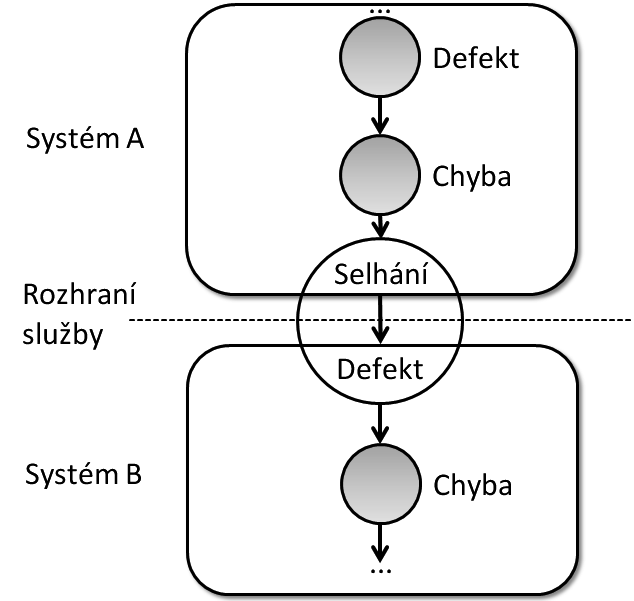
\includegraphics[width=8cm]{img/Bug.png}
	\end{figure}
	
	\section{Testování softwaru}
	Definice pojmu testování softwaru se více či méně liší téměř v~každé publikaci. V~knize \citep{RizeniKvalitySW} je testování definováno jako proces řízeného spouštění softwarového produktu s~cílem zjistit, zda splňuje specifikované či implicitní potřeby uživatelů. Je zde důležité slovo spouštění, které z~testování vyřazuje metody statické analýzy. Obecněji se však i~tyto metody do testovaní řadí a~jejich použití bývá ve vývoji softwaru vhodné.
	
	Záměrem testování již není nalézat defekty, jak tomu bylo dříve. Nyní je jím získat informaci o~kvalitě softwaru a~o~tom, jak moc splňuje požadavky zákazníka.
	
	\citep{Patton} uvádí řadu axiomů (obecně přijímaných pravd, které se nemusejí dokazovat) o~testování. Čtyři nejdůležitější z~nich jsou:
		\begin{itemize}
			\item Žádný program není možné otestovat kompletně -- počet vstupů, výstupů a~cest, které vedou skrze software je příliš velký.
			\item Testování softwaru je postavené na riziku -- nemožnost otestování všech případů vede k~tomu, že je možné nezachytit defekt ve scénáři, který se netestoval. Je proto důležité správně odhadnout možná rizika a~testováním je minimalizovat.
			\item Testování nikdy nemůže prokázat, že chyby neexistují -- testováním pouze můžeme dokázat, že chyby existují, ale jelikož není možné software kompletně otestovat, existenci chyb vyloučit nelze.
			\item Čím více chyb najdeme, tím více jich v~softwaru je -- kvůli tomu, že programátoři mívají špatné dny nebo dělají často stejné chyby, se chyby vyskytují ve skupinách. To znamená, že objevení jedné chyby zvyšuje pravděpodobnost dalších takových podobných chyb.
		\end{itemize}
		
		\section{Úrovně testování}
		Během vývoje softwaru se testování nechá rozdělit do různých skupin, např. podle toho, kdy se testování provádí, jakým způsobem se provádí, jak se k~testované aplikaci přistupuje, či jaká část aplikace se podrobuje testům. Rozlišují se např. tyto čtyři fáze:
			\begin{itemize}
				\item Testování jednotek (Unit Testing) -- testování provádí obvykle sám programátor, který se snaží prokázat správnost fungování jednotlivých jednotek (nejmenších testovatelných součástí aplikace).
				\item Integrační testování (Integration Testing) -- testuje se zapojení výše uvedených jednotek do aplikace. Správná funkčnost jednotek nezaručuje správnou funkčnost výsledné aplikace.
				\item Systémové testování (System Testing) -- testuje se, zda aplikace splňuje požadavky zákazníka. Patří sem nejen funkční testování, ale i~mimofunkční.
				\item Akceptační testování (User Acceptance Testing, UAT) -- zde provádí testování sám zákazník a~neomezuje se pouze na testování jako takové, ale na splnění před dohodnutých kritérii (dokumentace, manuály apod.).
			\end{itemize}
			
		\section{Testování uživatelského rozhraní}
		Podle \citep{Patton} má každá aplikace uživatelské rozhraní (UI -- user interface). V~dnešní době je dělíme do dvou skupin, grafické (GUI -- graphical user interface) a~z~příkazové řádky (CLI -- command line interface). V~obou případech UI slouží pro interakci a~komunikaci s~uživatelem. Je to prostředek pro zadávání vstupních data a~získávání výstupů.
		
		Použitelnost UI znamená, nakolik funkční a~efektivní je práce uživatele s~programem. K~tomu se vztahuje pojem ergonomika -- zabývá se návrhem a~konstrukcí předmětů s~ohledem na to, aby se s~nimi pracovalo jednoduše. Vzhledem k~použitelnosti se tedy bude testovat, zda je aplikace těžko srozumitelná, obtížně se s~ní pracuje, je pomalá, nebo ji zákazník nebude považovat za vyhovující.
		
		Dobré uživatelské rozhraní by mělo mít následující vlastnosti:
			\begin{itemize}
				\item Dodržuje standardy nebo zásady -- pokud aplikace poběží na specifické platformě, je možné, že pro tuto platformu existují předepsané standardy a~normy na vzhled a~chování aplikací (tzv. look and feel), které je vhodné dodržovat.
				\item Je intuitivní -- míry intuitivnosti softwaru jsou např.: Je UI zřetelné, vhodně rozložené? Nepřekáží vám v~tom, co s~ním hodláte dělat? Nachází se funkce a~odpovědi tam, kde je očekáváte? Je jasné, co bude další akce v~pořadí? Není příliš komplikované (neobsahuje moc funkcí)?
				\item Je konzistentní -- uživatelé si zvyknou na určitý způsob ovládání a~očekávají, že provedou stejnou akci velmi podobně i~v~jiném programu. Proto je důležité věnovat pozornost nejen konzistenci v~rámci naší aplikace, ale i~vůči ostatním. Pozor bychom si měli dávat na klávesové zkratky, výběry z~nabídek, umístění tlačítek, výstupy aplikace apod.
				\item Je flexibilní -- uživatelé mají rádi možnost volby. I~v~jednoduchých programech typu kalkulačka bývá na výběr alespoň ze dvou rozložení -- standardního a~vědeckého. To ovšem znesnadňuje testování, proto by voleb nemělo být příliš mnoho.
				\item Je pohodlné -- software by neměl uživateli práci s~ním nijak znepříjemňovat. Je vhodné zaměřit se na náležitost (měl by působit dojmem, který odpovídá jeho záměru), ošetření chyb (upozornění před kritickou operací, návrat o~krok zpět aj.), rychlost zpracování (chybové hlášky zobrazovat dostatečně dlouho, uvést odhadovaný čas do dokončení).
				\item Je správné -- ověřuje se to, zda UI dělá to, co má. Pozornost by se měla věnovat marketingovým rozdílům (v~aplikaci nejsou oproti marketingovým dokumentům funkce navíc, nebo chybějící funkce), jazyku a~pravopisu, nesprávným médiím (různorodé ikony, zvuky a~jiné části UI).
				\item Je užitečné -- přispívají dané funkce zvýšení užitné hodnoty aplikace? Pomůže uživateli v~jeho práci s~aplikací? Nepodstatné funkce znamenají zbytečné testování navíc a~pro zákazníka mohou být špatné.
			\end{itemize}
		
		\section{Automatizace testování}
		Důvodem automatizace testování je zvýšení jeho efektivity. Manuální návrh, provedení a~analýza testů jsou časově náročné a~často velice monotónní práce. Testeři mohou jednak ušetřit čas, a~jednak se sníží pravděpodobnost chybného vykonání testu z~důvodu ztráty koncentrace testera v~důsledku jednotvárné činnosti. Dalším přínosem je průběžně se stále zvětšující sada regresních testů. Ty slouží k~otestování, zda nově přidaná funkcionalita či úprava aplikace nezpůsobuje chyby v~již funkčních částech.
		
		Funkcionální testování UI je jednou z~částí testování UI, která se nechá automatizovat. Existuje celá řada nástrojů, které umožňují simulování klikání a~psaní na klávesnici. Další částí vhodnou pro automatizaci je kontrola, zda GUI obsahuje všechny prvky, a~jestli je chování prvků konzistentní a~stejné, jako požadované. V~obou těchto disciplínách je pro testovací nástroj důležité, aby zvládal klikat a~psát do aplikace, ale zároveň vyhodnocoval její stav (vstup je možné zadávat až tehdy, když je na to aplikace připravená, apod.).
		
			\subsection{Monkey testování}\label{MonkeyTestovani}
			Specifickou oblastí testování GUI a~automatického testování je tzv. monkey testování (testování za pomoci \emph{cvičené opice}). To vychází z~\uv{Nekonečného opičího teorému}, \citep{Patton}, \citep{Teorem}, který říká: \uv{Pokud bychom měli po nekonečnou dobu k~dispozici nekonečně mnoho opic, které by neustále náhodně psaly na nekonečně mnoho klávesnic, statisticky vzato by mohly nakonec napsat všechny Shakespearovy hry.}
			
			Nejde o~automatizaci za účelem usnadnění práce a~zvýšení efektivity, ale za účelem napodobit možné chování potenciálního uživatele. Přes všechno naše snažení a~testování určitě v~aplikaci zůstaly chyby, které by odhalil případný uživatel podobným nezasvěceným klikáním a~psaním. Tomu je však možné alespoň částečně předejít pomocí monkey testování.

\chapter{Přehled nástrojů}
V~této kapitole následuje přehled nástrojů a~některých jejich vlastností. V~tabulce \ref{PrehledNastroju} je uveden název nástroje, jeho licence resp. cena, jazyk, ve kterém se testy píší, platforma, na které nástroj funguje a~která GUI je nástroj schopen testovat. Z~bezplatných multiplatformních nástrojů jsem si vybral tři a~ty podrobněji prozkoumal a~porovnal, viz následující kapitola.
{\scriptsize
\begin{longtable}{|l|l|l|l|l|l|}
		\hline
		\textbf{Název}&\textbf{Licence/Cena}&\textbf{Skriptovací jazyk}&\textbf{Platforma}&\textbf{\shortstack{\\Jazykové\\omezení}}\\\hline\hline
		AutoIt \cite{AutoIt}&Freeware&BASIC-like&Windows&-\\\hline
		AutoHotKey \citep{AutoHotKey}&GNU GPLv2&AutoHotKey&Windows&-\\\hline
		AutoKey \citep{AutoKey}&GNU GPLv3&Python&Linux&-\\\hline
		\shortstack{\\SikuliX \citep{Sikuli}\\\citep{SikuliX}}&MIT License&Python, Ruby&\shortstack{\\Windows,\\Linux, Mac}&-\\\hline
		Jubula \citep{Jubula}&EPL 1.0&\shortstack{\\Drag \& Drop,\\Java}&\shortstack{\\Windows,\\Linux, Mac}&\shortstack{\\Java, HTML,\\.NET, iOS} \\\hline
		\shortstack{Robot\\Framework\\\citep{RobotFramework}}&\shortstack{Apache\\License 2.0}&Natural-like&\shortstack{\\Windows,\\Linux, Mac}&\shortstack{\\Podle pluginů\\(Java, web,\\Android, iOS,\\\dots)}\\\hline
		Squish \citep{Squish}&\shortstack{\\cca\\\EUR{2400}/osoba}&\shortstack{\\Python, JavaScript,\\Ruby, Perl, Tcl}&\shortstack{\\Windows,\\Linux, Mac}&-\\\hline
		eggPlant \citep{eggPlant}&\shortstack{\\nedostupná,\\vázaná na stroj}&\shortstack{\\SmartTalk,\\Drag \& Drop,\\pomocí rozhraní\\eggDrive např.\\Java, C\#, Ruby}&\shortstack{\\Windows,\\Linux, Mac}&-\\\hline
		UFT \citep{UFT}&nedostupná&\shortstack{\\VBScript,\\Drag \& Drop}&\shortstack{\\Windows,\\Linux, Mac}&-\\\hline
		\shortstack{\\Rational\\Functional\\Tester} \citep{RFT}&3300 \$/osoba&Nahrávání akcí&\shortstack{\\Windows,\\Linux}&-\\\hline
		Ranorex \citep{Ranorex}&\EUR{690}&\shortstack{\\C\#, VisualBasic,\\nahrávání akcí}&Windows&-\\\hline
		SilkTest \citep{SilkTest}&nedostupná&\shortstack{\\C\#, VisualBasic,\\Java}&Windows&-\\\hline
		\shortstack{\\TestComplete\\\citep{TestComplete}}&\EUR{889 }/stroj&\shortstack{\\Python, VBScript,\\JScript, C\#Script,\\DelphiScript,\\C++Script,\\nahrávání akcí}&Windows&-\\\hline
	\captionsetup{font=normalsize}
	\caption{Přehled nástrojů}
	\label{PrehledNastroju}
\end{longtable}
}

\chapter{Zvolené nástroje}
Vzhledem k~požadavkům na nástroje, které vyplývají z~vazby na předmět KIV/OKS, jako je bezplatnost, schopnost fungování nezávisle na OS nebo podpora testování programů vytvořených technologií Java a~webových aplikací, jsem z~výše zmíněných vybral nástroje Jubula, SikuliX a~Robot Framework. Každý z~nástrojů bude stručně charakterizován a~bude následovat podrobnější srovnání.
	\section{Jubula}
	Jubula je nástroj, který vznikl a~je vyvíjen v~rámci IDE Eclipse. Do projektu přispívá také firma BREDEX GmbH, která vytváří i~tzv. standalone verzi, což je program, který je možné používat samostatně bez IDE Eclipse. Navíc obsahuje navíc některé nespecifikované funkce a~nemusí být licencována pod EPL 1.0, jako je tomu u~verze pro IDE Eclipse.
	
	Pro tvorbu testovacích skriptů byla používána metoda Drag \& Drop, popř. se akce určovaly klikáním na různé nabídky. V~jedné z~posledních verzí bylo vydáno Java API a~skripty je tak možné psát pomocí jazyka Java. Mezi podporovaná testovaná rozhraní patří Java Swing, SWT, JavaFX, HTML a~iOS. Výhodou této aplikace je také možnost její integrace do ostatních programů pro organizaci testování.
	
	\section{SikuliX}
	Sikuli (nověji SikuliX) je nástroj, který vznikl jako projekt skupiny User Interface Design Group na MIT, což odpovídá i~jeho licenci -- MIT License. Nyní jeho vývoj převzal Raimund Hock (aka RaiMan) společně s~open-source komunitou.
	
	Při tvorbě skriptů je možné využít pro SikuliX vlastní jazyk podobný přirozené angličtině, nebo některý ze zavedených, jako je Python, Ruby, Java, Jython, JRuby, Scala, Groovy, Clojure a~další. Nástroj není omezený na určitá testovaná rozhraní, protože k~identifikaci GUI používá rozpoznávání obrazu podle vzoru\footnote{Pomocí OpenCV, \url{http://opencv.org/}}, dokáže simulovat ovládání myši a~klávesnice nebo rozpoznávat text v~obrázcích\footnote{Pomocí Tesseract OCR, \url{https://github.com/tesseract-ocr}}. Výhodou této aplikace je proto její nezávislost vůči testovanému rozhraní. Cenou za to je pravděpodobné snížení její rychlosti. Použití SikuliX se neomezuje pouze na testování, ale je možné pomocí něj i~automatizovat činnosti.
	
	\section{Robot Framework}
	Robot Framework je nástroj založený na pluginech a~je open-source. Vývoj podporuje společnost Nokia Networks.
	
	Základ nástroje, tzv. core framework, je vytvořený v~jazyce Python. Knihovny je možné psát v~jazyce Python nebo Java a~samotné skripty pak v~jazyce podobném přirozené angličtině. Díky dodržování jistého formátování je pro člověka velmi přehledný. Mezi podporovaná testovaná rozhraní patří např. Android, iOS, Java Swing, webové aplikace, databáze a~aplikace vytvořené pro OS Windows. Výhodou této aplikace je možnost si chybějící modul pro testování určitého rozhraní vytvořit a~používat.

\chapter{Srovnání nástrojů}
Pro srovnání nástrojů byl vytvořen návrh multikriteriálního hodnocení, který se snaží nástroje hodnotit z~různých úhlů a~vytvořit tak komplexní klasifikaci. Každé z~hodnocených částí je možné přiřadit vlastní váhu. Ta určuje důležitost hodnotícího kritéria pro každého jedince a~tím napomáhá výběru vhodného nástroje. V~obrázku \ref{MKHodn} je návrh ukázán a~je vidět výsledek pro mnou zvolené váhy, viz obrázek \ref{MKVysl}. Jako nejvhodnější se jeví použití nástroje SikuliX. Dále se budu věnovat jednotlivým hodnotícím kritériím.

Možnost vytváření testů je jedno z~nejdůležitějších kritérií vzhledem k~vazbě na předmět KIV/OKS. Hlavním požadavkem bylo, aby bylo možné testy tvořit v~jazyce Java. Dále jsem vybral několik skriptovacích jazyků a~metod.

Podpora testovaných rozhraní byla dalším z~rozhodujících kritérií. Hlavními platformami měly být aplikace vytvořené pomocí jazyka Java a~webové aplikace. Opět jsem přidal některé další běžné platformy. Nástroj by měl být též multiplatformní, proto je jedním z~kritérií podpora operačních systémů.

Reportování výsledků testů, složitost jejich tvorby a~jejich přehlednost může napomoci vývojáři diagnostikovat případnou chybu. Také je přínosné znát stav obrazovky a~to zajistí screenshot. Díky tomu se stává vývoj jednodušší, a~proto jsem toto kritérium také zařadil do hodnocení.

Dále jsem přidal kritérium univerzálnosti nástroje s~poněkud individuálním ohodnocením. To je zde myšleno tak, co obecně nástroj dokáže, ale co není podstatné z~pohledu předmětu KIV/OKS. Například Jubula je čistě testovací nástroj, ale SikuliX se dá použít navíc pro automatizaci pracovních postupů.

Posledním kritériem je vhodnost nástroje pro účely předmětu KIV/OKS. Jedná se hlavně o~to, jak zapadá do konceptu výuky, jak je práce s~ním složitá a~jaké má nároky na studentovy znalosti.
\\[\topsep]Vysvětlivky termínů z~dále použitých tabulek:
\vspace{-\topsep}
\begin{itemize}
	\item Natural-like -- víceméně okleštěný přirozený jazyk založený na angličtině,
	\item Složitost tvorby -- míní se tím složitost přípravy reportu a~v~tabulce vyšší počet bodů znamená jednodušší tvorbu pro tvůrce skriptů
\end{itemize}
\begin{figure}[ht!]
	\begin{subfigure}{\textwidth}
		\centering
		\caption{Multikriteriální hodnocení}
		\label{MKHodn}
		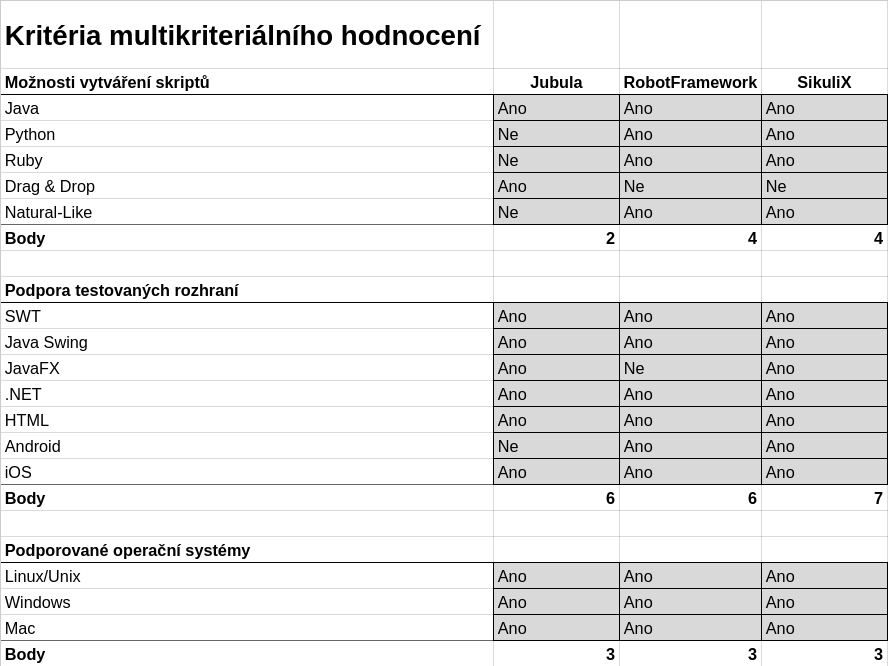
\includegraphics[width=13.5cm]{img/Kriteria/Kriteria1.png}
		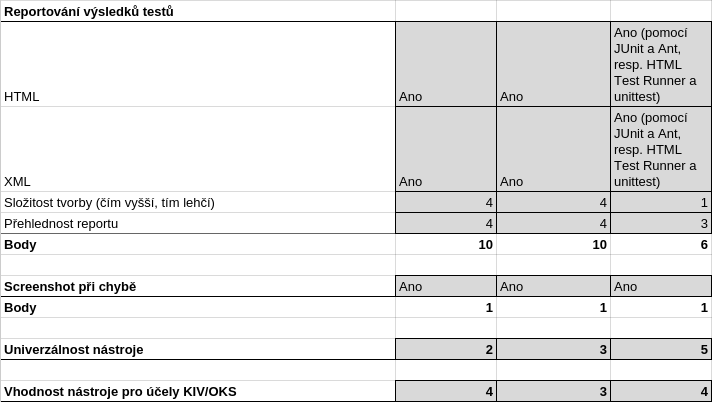
\includegraphics[width=13.5cm]{img/Kriteria/Kriteria2.png}
	\end{subfigure}
\end{figure}
\begin{figure}[ht!]
	\ContinuedFloat
	\begin{subfigure}{\textwidth}
		\centering
		\caption{Výsledek multikriteriálního hodnocení}
		\label{MKVysl}
		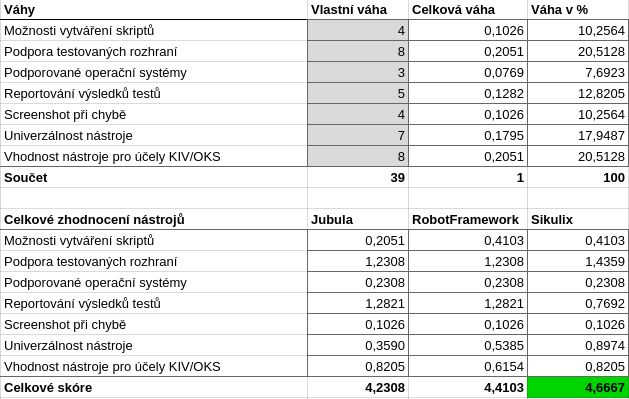
\includegraphics[width=13.5cm]{img/Kriteria/Kriteria3.png}
	\end{subfigure}
\end{figure}

Z~uvedeného multikriteriálního hodnocení je zřejmé, že vybrané nástroje jsou v~podstatě vyrovnané. To ostatně potvrzuje i~jejich poměrné zastoupení mezi uživateli. SikuliX byl zvolen též po diskuzích s~vedoucím práce a~to pro jeho vlastnost naprosté nezávislosti na testovaném rozhraní. Tato vlastnost se významně hodí v~předmětu KIV/OKS, protože je možné dát nástroj do kontrastu s~nástrojem Selenium. Jinými slovy řečeno SikuliX je principiálně odlišný nástroj, což není možné říci o~např. Jubule.

\chapter{SikuliX}
	\section{Instalace}
	Po stažení balíčku započne instalace jeho spuštěním\footnote{Je potřeba instalace JRE nebo JDK 6 a~vyšší, v~linuxové distribuci balíky \emph{libopencv-core2.4, libopencv-imgproc2.4, libopencv-highgui2.4, libtesseract3} a~\emph{wmctrl} \citep{SikuliX}}. Je ukázána instalace v~Linuxu, avšak instalace ve Windows je obdobná. V~průběhu máme na výběr různé možnosti, jak chceme nástroj používat, viz obrázek \ref{Instal}. Např. zda chceme používat SikuliX-IDE a~Python nebo Ruby, jestli budeme používat jiné IDE a~Javu a~zda chceme používat OCR\footnote{Optical Character Recognition -- optické rozpoznání znaků} funkce. Zaškrtneme všechna políčka kromě \emph{Ruby (JRuby)} a~klikneme na \emph{Setup Now}. Jsme dotázáni, zda chceme balíčky stáhnout, nebo ukončit instalaci. Zvolíme \emph{Yes}. Další dotaz je na verzi Jythonu, kterou chceme použít, s~upozorněním, že může nastat problém se znaky v~kódování UTF-8. Opět zvolíme \emph{Yes}. Začne vytváření souborů a~měla by se otevřít dvě okna jako na obrázu \ref{InstalOK}, obě potvrdíme tlačítkem \emph{OK}. Pokud vše proběhne v~pořádku, vzniknou v~adresáři soubory podobné těmto\footnote{Může se lišit na různých OS} \emph{runsikulix, SetupStuff, SikuliX-1.1.0-SetupLog.txt, sikulixapi.jar, sikulix.jar}.
	\begin{figure}[ht!]
		\centering
		\caption{Instalace SikuliX}
		\label{Instal}
		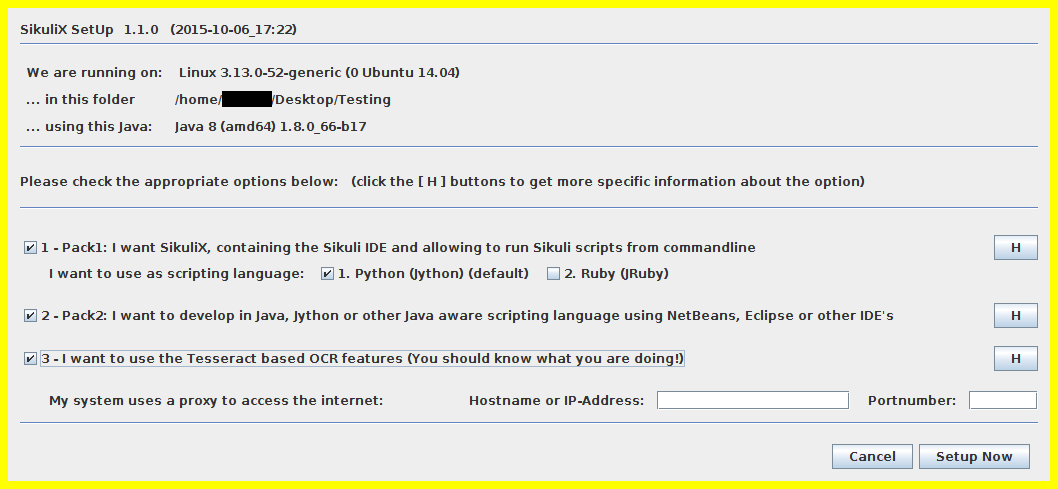
\includegraphics[width=13.5cm]{img/Instalace/Instalace.png}
	\end{figure}
	\begin{figure}[ht!]
		\centering
		\caption{Test instalace}
		\label{InstalOK}
		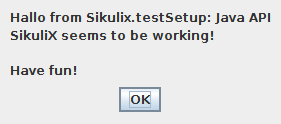
\includegraphics[width=8cm]{img/Instalace/InstalaceOK.png}\\[0.3cm]
		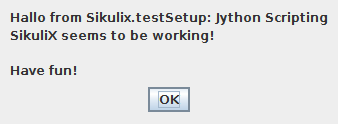
\includegraphics[width=8cm]{img/Instalace/InstalaceOK1.png}
	\end{figure}
	
	\section{Tvorba testů}
	Budeme pracovat s~webovou aplikací \emph{Převodník} dostupné z~url \url{http://oks.kiv.zcu.cz/Prevodnik/Prevodnik}. V~té se vyskytují záměrné chyby a~bude sloužit jako cvičná aplikace pro tuto práci.
	
	Pro tvorbu testů pomocí SikuliX jsou nejdůležitější snímky (screenshoty) řídících prvků, které bude SikuliX hledat a~případně používat k~některým akcím. Je tedy vhodné si nejprve aplikaci spustit, vybrat příslušné prvky a~vytvořit jejich snímky. Při jejich tvorbě se doporučuje preciznost a~přesnost, neboť v~jistých situacích mohou nastat problémy, které budou zmíněny později.
	
	Pokud je snímků více, je vhodné je třídit do adresářů. To není nutné, ale zlepšuje to čitelnost kódu a~usnadňuje práci s~nástrojem. Adresáře mohou např. sdružovat snímky prvků, které jsou si nějakým způsobem podobné (tlačítka, textová pole, výběrové seznamy, chybové hlášky, apod.). Stejně tak je vhodné snímky pojmenovávat na základě toho, co obsahují (vstupní textové pole, label Vstup, apod.).
	
	Dle \citep{SikuliXImgs} SikuliX interně používá třídu ImageIO z~Javy. Podporované formáty jsou tedy bmp, wbmp, jpg, jpeg, png a~gif. Vzhledem k~vlastnostem se doporučuje používat formát png.
	
	Pokud je vytvářený test jednoduchý a~není potřeba většího množství testů, je jednodušší vytvořit jej pomocí SikuliX-IDE. Pokud však chceme aplikaci testovat podrobněji a~psát velké množství testovacích případů, je vhodnější použít některý z~podporovaných programovacích jazyků a~využít tak jeho možnosti jako nadstavbu nad SikuliX.
	
	\section{SikuliX-IDE}
	Dle \citep{SikuliX} je možné SikuliX-IDE spustit různými způsoby:
	\begin{enumerate}
		\item Spuštěním souboru \emph{SikuliX.app} (Mac) nebo \emph{SikuliX.exe} (Windows),
		\item dvojklikem na soubor \emph{runsikulix} (Linux) nebo \emph{runsikulix.cmd} (Windows),
		\item z~příkazové řádky příkazem\\
		\texttt{java -jar cesta/k/sikulix.jar [volitelne parametry]}
	\end{enumerate}
	Po spuštění vypadá IDE jako na obrázku \ref{SikuliXIDE}. Jako parametry se v~metodách, ve kterých je to možné, ukazují obrázky vzorů, podle kterých se na obrazovce nástroj orientuje, případně cesta k~nim.
	\begin{figure}[ht!]
		\centering
		\caption{SikuliX-IDE}
		\label{SikuliXIDE}
		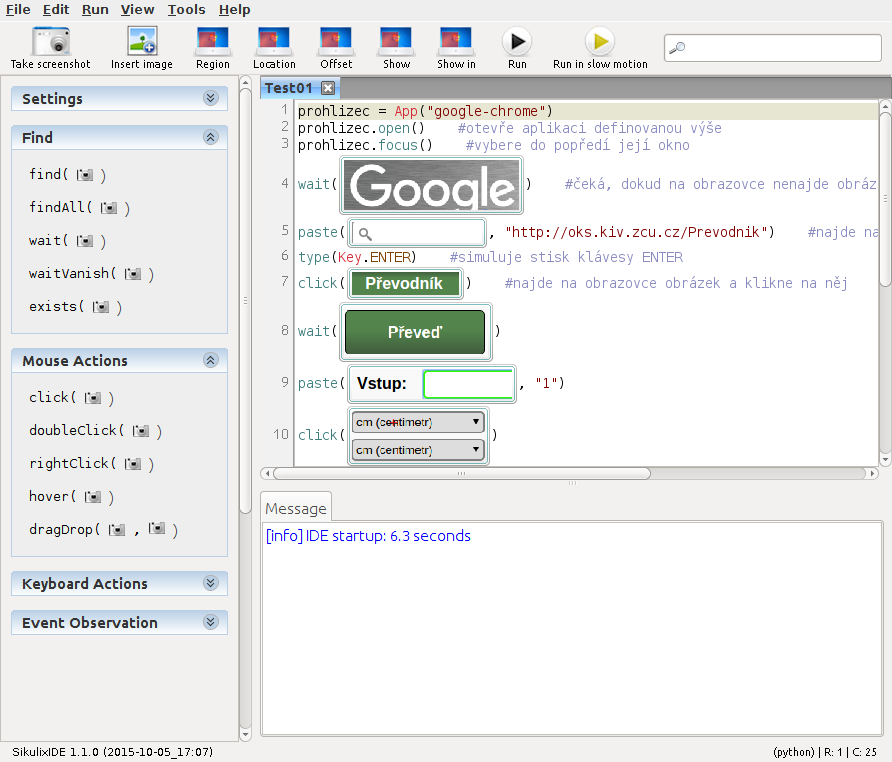
\includegraphics[width=13.5cm]{img/SikuliXIDE.png}
	\end{figure}
	
		\subsection{První skript}
		Skript se připravuje v~SikuliX-IDE, které je vidět na obrázku \ref{SikuliXIDE}. Kód, který je vidět v~\ref{PrvniSkript}, nemusí být v~IDE identický, ale cesta k~obrázku může být nahrazena jeho náhledem, pokud je tato možnost zvolena v~nastavení nástroje. K~tvorbě jsou v~IDE užitečné pomůcky, které se nacházejí v~levém a~v~horním panelu.
		
		Pro spuštění aplikace (např. webového prohlížeče) se do příslušné metody zadá cesta k~jeho spustitelnému souboru. Pokud se používá OS Linux, stačí zadat terminálový příkaz pro spuštění (např. \texttt{"google-chrome"}, \texttt{"firefox"}, apod.).
		
		Skript pracuje tak, že se otevře prohlížeč, který přejde na adresu \url{http://oks.kiv.zcu.cz/Prevodnik}. Klikne na odkaz \emph{Převodník}, do vstupního pole vloží \emph{1} a~stiskne \emph{Převeď}. Z~pole s~výsledkem přečte text a~porovná jej s~předpokládanou hodnotou \emph{2,54}. Pokud si odpovídají, objeví se dialogové okno s~potvrzením, jestliže ne, zobrazí se chybová hláška. Obdobně je tomu v~následující části, kde se pouze kontroluje existence obrázku.
		\\[\topsep]Pro vytvoření skriptu postupujeme následovně:
		\vspace{-\topsep}
			\begin{enumerate}
				\item Spustíme SikuliX-IDE jednou z~výše uvedených metod.
				\item Napíšeme kód pro otevření a~vybrání okna prohlížeče do popředí:\\\texttt{prohlizec = App("google-chrome")\\prohlizec.open()\\prohlizec.focus()}
				\item Spustíme prohlížeč.
				\item V~SikulixIDE v~levém menu klikneme na 
\includegraphics[scale=0.7]{img/PrvniSkript/wait.png} a~provedeme screenshot statické části aplikace. Skript tedy bude vypadat přibližně takto:
					\begin{figure}[ht!]
						\centering
						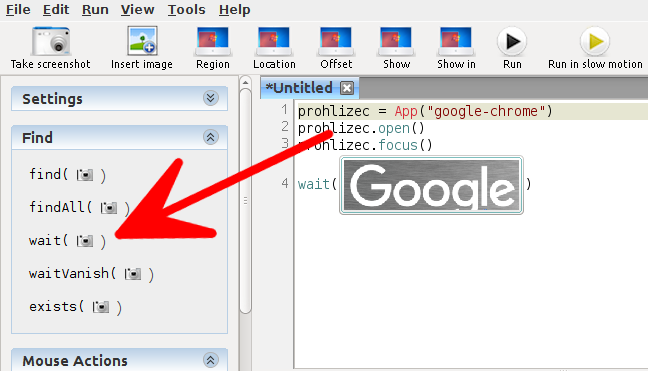
\includegraphics[width=12.5cm]{img/PrvniSkript/krok4.png}
					\end{figure}
					\FloatBarrier
				\item V~levém menu otevřeme podmenu \emph{Keyboard Actions} a~vybereme\\
\includegraphics[scale=0.7]{img/PrvniSkript/paste.png}. Nyní provedeme screenshot políčka pro URL adresu a~jako druhý parametr funkce zadáme URL adresu aplikace \emph{Převodník} (\url{"http://oks.kiv.zcu.cz/Prevodnik"}). Přidaná část tedy vypadá přibližně takto:
					\begin{figure}[ht!]
						\centering
						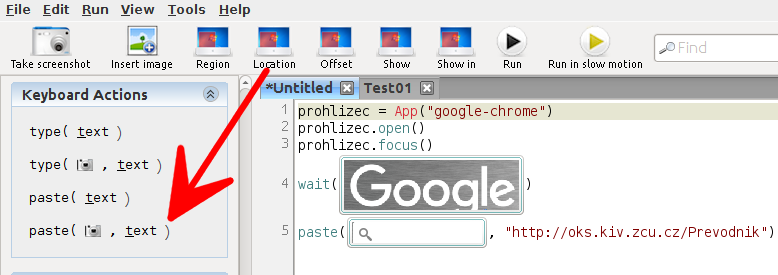
\includegraphics[width=12.5cm]{img/PrvniSkript/krok5.png}
					\end{figure}
					\FloatBarrier
				\item Na další řádku zadáme příkaz pro stisknutí klávesy Enter:\\\texttt{type(Key.ENTER)}
				\item V~prohlížeči otevřeme webovou stránku s~aplikací \emph{Převodník}. V~SikuliX-IDE klikneme v~levém menu na 
\includegraphics[scale=0.7]{img/PrvniSkript/click.png} a~provedeme screenshot záložky, která odkazuje na \emph{Převodník}.
					\begin{figure}[ht!]
						\centering
						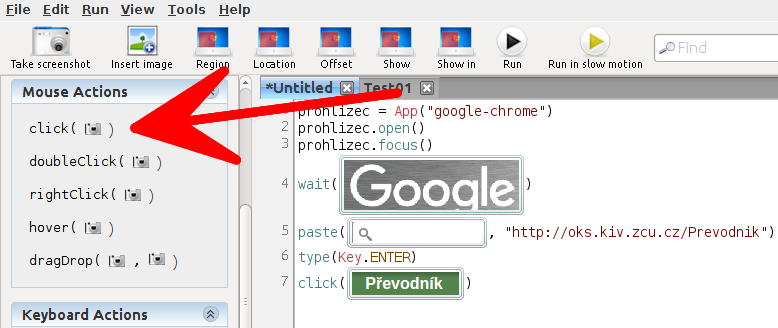
\includegraphics[width=12.5cm]{img/PrvniSkript/krok7.png}
					\end{figure}
					\FloatBarrier
				\item Klikneme na záložku aplikace \emph{Převodník}. V~SikuliX-IDE opět vybereme 
\includegraphics[scale=0.7]{img/PrvniSkript/wait.png} a~uděláme snímek tlačítka \emph{Převeď}.
				\item Dále vybereme 
\includegraphics[scale=0.7]{img/PrvniSkript/paste.png} a~vytvoříme snímek vstupního pole. Snímek musí obsahovat popisek \emph{Vstup:}, aby byl jednoznačně identifikovatelný. Také musí obsahovat část vstupního pole dost velkou na to, aby ve středu snímku bylo toto pole, nikoli jeho okolí. Vložení hodnoty se provádí do středu snímku, což se ovšem dá upravit, jak si ukážeme v~dalším kroku. Jako druhý parametr zadáme hodnotu \texttt{"1"}.
				\item Vybereme možnost 
\includegraphics[scale=0.7]{img/PrvniSkript/click.png} a~vytvoříme screenshot obou výběrových seznamů. Nyní klikneme na obrázek seznamů v~SikuliX-IDE a~otevře se okno:
					\begin{figure}[ht!]
						\centering
						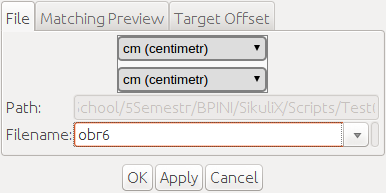
\includegraphics[width=10.5cm]{img/PrvniSkript/pattern.png}
					\end{figure}
					\FloatBarrier
					Klikneme na \emph{Target Offset}, které vypadá následovně:
					\begin{figure}[ht!]
						\centering
						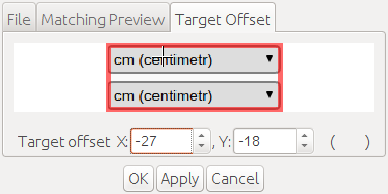
\includegraphics[width=10.5cm]{img/PrvniSkript/offset.png}
					\end{figure}
					\FloatBarrier
					Zde buď zadáme příslušné hodnoty do vstupních políček, nebo jen vybereme v~obrázku požadované místo. To nám zajistí, že SikuliX neklikne do středu obrázku, ale na zvolené místo v~něm. Potvrdíme tlačítkem \emph{OK} a~pokračujeme v~tvorbě skriptu.
				\item Nyní nastává problém. Potřebujeme vytvořit screenshot jedné položky ve výběrovém seznamu, ale SikuliX-IDE nám k~tomu nedává možnost. Řešením je např. v~prohlížeči výběrový seznam rozbalit, provést screenshot celé obrazovky pomocí tlačítka \emph{PrintScreen} a~v~nějakém grafickém editoru vyříznout pouze tu část, kterou chceme (
\includegraphics[scale=0.8]{img/PrvniSkript/inch.png}). Tu poté uložíme do složky s~vytvářeným skriptem a~pouze doplníme následující kód: \texttt{click("nazev-snimku.png")}
				\item Na novou řádku napíšeme kód \texttt{click()} a~do závorek zkopírujeme výše použitý obrázek tlačítka \emph{Převeď}.
				\item Na další řádce si vytvoříme proměnnou \emph{vystup} a~přiřadíme do ní text z~výstupního textového pole. To se provede následujícím způsobem:\\\texttt{vystup = find("label-vystup.png").right(100).text()}\\
				Funkce \emph{right()} říká, že pracujeme s~oblastí širokou 100 pixelů napravo od nalezeného obrázku (popisku \emph{Výstup:}). Funkce \emph{text()} provede OCR a~vrátí zjištěný text.
					\begin{figure}[ht!]
						\centering
						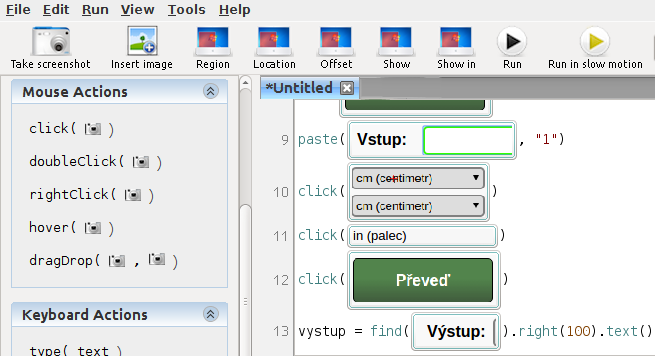
\includegraphics[width=12.5cm]{img/PrvniSkript/krok13.png}
					\end{figure}
					\FloatBarrier
				\item V~další části provedeme kontrolu zjištěného textu. Ten má obsahovat výslednou hodnotu -- 2.54. Vložíme do programu následující úsek kódu:\\\texttt{if vystup == "2.54":
					\\{\setlength{\parindent}{1cm}\indent popup("Ok textově")}
				\\else:
					\\{\setlength{\parindent}{1cm}\indent popError("Chyba")}}
				\item Další následuje \uv{optická} kontrola podle screenshotu. Potřebujeme si připravit do výstupního textového pole správný výsledek (hodnotu 2.54). To lze např. udělat tak, že provedeme převod hodnoty 2.54 mezi stejnými jednotkami. Jakmile se nám toto podaří, uděláme snímek výsledku a~uložíme jej ke skriptu. Zkopírujeme kód z~bodu 16. a~upravíme if-větev tak, že smažeme porovnání proměnné s~hodnotou a~napíšeme jako podmínku následující: \texttt{exists("nazev-snimku.png")}.
					\begin{figure}[ht!]
						\centering
						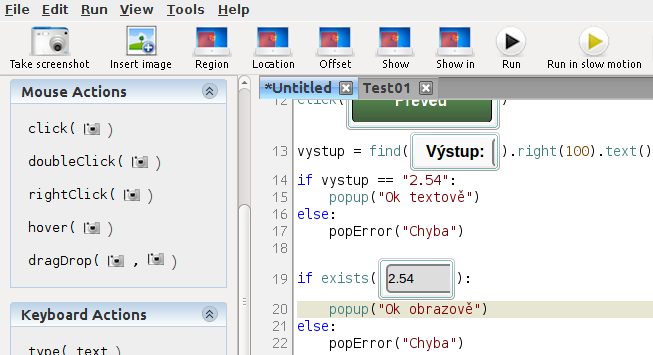
\includegraphics[width=12.5cm]{img/PrvniSkript/krok15.png}
					\end{figure}
					\FloatBarrier
				\item Jako poslední bod je zavření prohlížeče. To se provede příkazem\\\texttt{prohlizec.close()}.
			\end{enumerate}
			Tímto postupem by měl vzniknout skript téměř totožný s~tím, který je uveden v~kódu \ref{PrvniSkript}. Nebude obsahovat komentáře a~mohou se lišit názvy snímků.
		
			\begin{lstpython}{caption={První skript}, label={PrvniSkript}}
prohlizec = App("google-chrome")
prohlizec.open()	#otevre aplikaci definovanou
				#vyse
prohlizec.focus()	#vybere do popredi jeji okno
#ceka, dokud na obrazovce nenajde obrazek
wait("obr1.png")
#najde na obrazovce obrazek a vlozi do neho text
paste("obr2.png", "http://oks.kiv.zcu.cz/Prevodnik")
type(Key.ENTER)	#simuluje stisk klavesy ENTER
#najde na obrazovce obrazek a klikne na nej
click("obr3.png")
wait("obr4.png")
paste("obr5.png", "1")
#klikne o 27px vyse a 18px vlevo od nalezeneho
#obrazku
click(Pattern("obr6.png").targetOffset(-27,-18))
click("obr7.png")
click("obr4.png")
#precte text z casti, ktera je 100px vpravo od
#nalezeneho obrazku
vystup = find("obr8.png").right(100).text()
if vystup == "2.54":
	#pokud rozpoznany text souhlasi se zadanym,
	#otevre se vyskakovaci okno
    popup("Ok textove")
else:
    popError("Chyba")    #jinak se zobrazi chybove
    			 #okno

if exists("obr9.png"):
	#pokud na obrazovce existuje obrazek, otevre
	#se vyskakovaci okno
    popup("Ok obrazove")
else:
    popError("Chyba")
prohlizec.close()    #ukonci aplikaci
\end{lstpython}
		
	\section{Java API}
	Dále bylo zkoumáno Java API, které SikuliX poskytuje. Pro jeho použití je potřeba mít při překladu a~spuštění nastavený v~classpath \emph{sikulixapi.jar}. Toho docílíme např. tak, že použijeme v~příkazové řádce dvou příkazů\\\texttt{javac -cp sikulixapi.jar:. Test01.java}\\\texttt{java -cp sikulixapi.jar:. Test01}\\ Syntaxe, kterou SikuliX v~Java API využívá, je velmi podobná té v~SikuliX-IDE.
	
		\subsection{První test}
		První test s~použitím Java API, viz kód \ref{PrvniJavaAPI}, je téměř identický s~tím, který byl vytvořen pomocí SikuliX-IDE.
		
			\begin{lstjava}{caption={První test Java API}, label={PrvniJavaAPI}}
import org.sikuli.basics.Settings;
import org.sikuli.script.*;
import javax.swing.*;

public class Test01 {

  static Screen s;
  static App prohlizec;
  
  public static void main(String [] args) {
    Settings.OcrTextSearch = true;
    Settings.OcrTextRead = true;

    s= new Screen();
    prohlizec = new App("google-chrome");
    prohlizec.open();
    prohlizec.focus();
    
    try {
      s.wait("obr1.png");
      s.paste("obr2.png");
      s.type(Key.ENTER);
      s.click("obr3.png");
      s.wait("obr4.png");
      s.paste("obr5.png", "1");
      s.click(new Pattern("obr6.png").targetOffset(
        -27,-18));
      s.click("obr7.png");
      s.click("obr4.png");
      String t = s.find("obr8.png").right(
        100).text();
      if (Double.parseDouble(t) == 2.54) {
        JOptionPane.showMessageDialog(null, "Ok" +
          " textove");
      } else {
        JOptionPane.showMessageDialog(null, "Chyba");
      }
      if (s.exists("obr9.png") != null) {
        JOptionPane.showMessageDialog(null, "Ok" +
          " obrazove");
      } else {
        JOptionPane.showMessageDialog(null, "Chyba");
      }
      prohlizec.close();
    } catch (Exception e) {
      e.printStackTrace();
    }
  }
}
\end{lstjava}
	
		\subsection{Sofistikovanější testy}
		S~využitím knihoven \emph{JUnit} a~\emph{Log4j} (ani jedna z~těchto knihoven není pro běh SikuliX bezprostředně nutná) byly vytvořeny čtyři testy, viz kód \ref{DalsiJavaAPI}. První test skončí negativně, druhý pozitivně, třetí pozitivně a~čtvrtý negativně.
		
		Knihovna \emph{JUnit} byla použita z~toho důvodu, že nám pomůže jednak s~organizací testů a~jejich spouštěním, a~jednak s~jejich vyhodnocováním. Dále obsahuje metody pro vyhodnocování a~porovnávání hodnot, tzv. \emph{asserty}.
		
		\emph{Log4J} je knihovna, která slouží k~logování informací do souborů. Umožňuje vlastní konfiguraci výstupních souborů a~spoustu dalších funkcí. Použita byla z~toho důvodu, že během testování je vhodné zaznamenávat prováděné činnosti z~důvodu jednoduššího zjištění případného selhání testu. SikuliX poskytuje informace o~tom, kam klikal či psal. Ty vypisuje na standardní výstup, avšak poskytuje metodu, které se předá instance \emph{Logger}, který poté SikuliX použije pro logování. Následuje ukázka zapisovaných informací, formátovaných vlastní konfigurací logeru, viz \ref{konfigurace}.
		{\lstset{basicstyle=\ttfamily\small}
		\begin{lstlisting}[]
18.04.2016 12:58:45 [INFO - TS03VymazaniJavaFX.
  invoke0()] - [info] runcmd: lsb_release -i -r -s
18.04.2016 12:58:46 [INFO - TS03VymazaniJavaFX.
  invoke0()] - [log] App.focus:  [1:PreVODNIK]
18.04.2016 12:58:50 [INFO - TS03VymazaniJavaFX.
  invoke0()] - [log] CLICK on L(925,298)@S(0)[0,0
  1920x1080]
18.04.2016 12:58:50 [INFO - TS03VymazaniJavaFX.
  invoke0()] - [log] CLICK on L(1128,298)@S(0)[0,0
  1920x1080]
18.04.2016 12:58:51 [INFO - TS03VymazaniJavaFX.
  invoke0()] - [log] CLICK on L(1128,422)@S(0)[0,0
  1920x1080]
18.04.2016 12:58:51 [INFO - TS03VymazaniJavaFX.
  invoke0()] - [log] CLICK on L(1128,333)@S(0)[0,0
  1920x1080]
18.04.2016 12:58:52 [INFO - TS03VymazaniJavaFX.
  invoke0()] - [log] CLICK on L(1127,457)@S(0)[0,0
  1920x1080]
18.04.2016 12:58:52 [INFO - TS03VymazaniJavaFX.
  invoke0()] - [log] CLICK on L(960,400)@S(0)[0,0
  1920x1080]
18.04.2016 12:58:53 [INFO - TS03VymazaniJavaFX.
  invoke0()] - [log] CLICK on L(960,587)@S(0)[0,0
  1920x1080]
18.04.2016 12:58:58 [ERROR - TS03VymazaniJavaFX.
  TC03_01_02PrevodChyba()] - Vstupni vyberovy seznam
  nema defaultni hodnotu
18.04.2016 12:58:59 [INFO - TS03VymazaniJavaFX.
  invoke0()] - [log] CLICK on L(661,198)@S(0)[0,0
  1920x1080]
	\end{lstlisting}}

\chapter{Sada ukázkových testů a~jejich scénářů}
Jak již bylo zmíněno dříve, existuje webová aplikace \emph{Převodník} dostupná z~url \url{http://oks.kiv.zcu.cz/Prevodnik/Prevodnik} se záměrnými chybami. Pro potřeby práce a~pro názornou ukázku odlišnosti přístupu k~testování webové a~desktopové aplikace byla vytvořena téměř identická aplikace Převodník pomocí technologie JavaFX, jejíž kód se nachází na přiloženém CD. Následující sada testů a~jejich scénářů se vztahuje k~těmto aplikacím, jejichž vzhled je ukázán na obrázcích \ref{PrevodnikWeb} a~\ref{PrevodnikJavaFX}.

	\begin{figure}[ht!]
		\centering
		\caption{Webová aplikace Převodník}
		\label{PrevodnikWeb}
		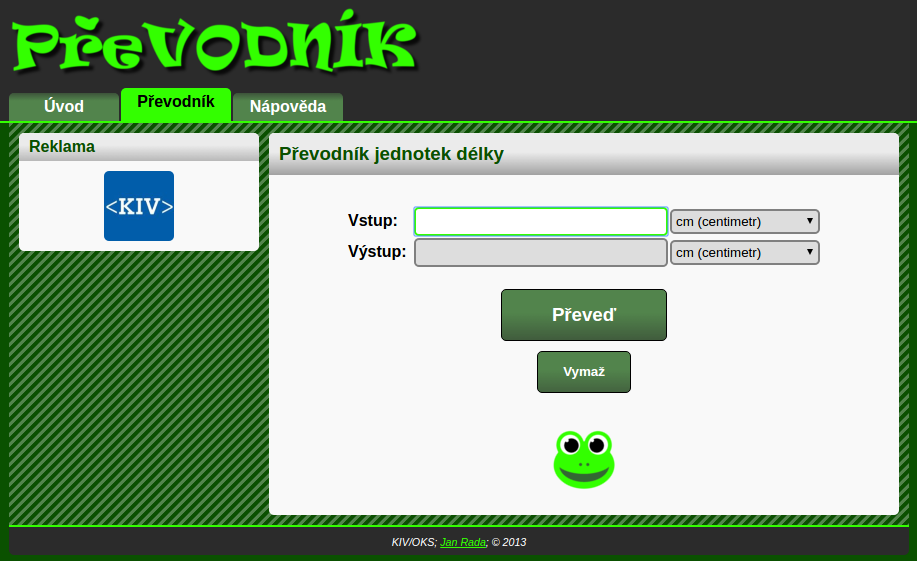
\includegraphics[width=13.5cm]{img/PrevodnikWeb.png}
	\end{figure}
	\begin{figure}[ht!]
		\centering
		\caption{Aplikace Převodník vytvořená pomocí JavaFX}
		\label{PrevodnikJavaFX}
		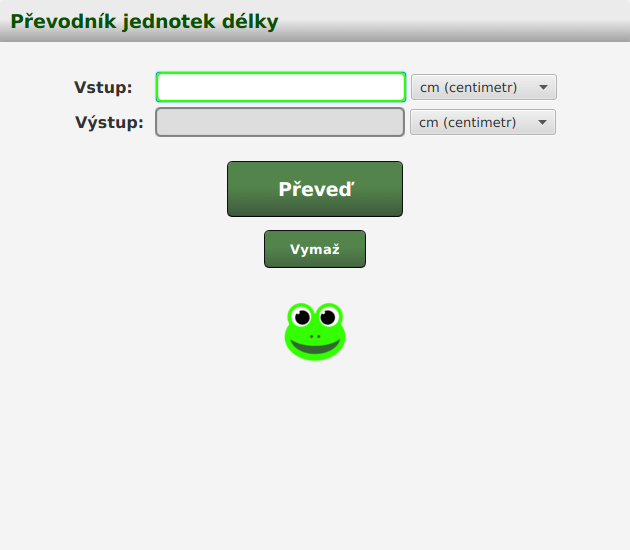
\includegraphics[width=13.5cm]{img/PrevodnikJavaFX.png}
	\end{figure}

Ze scénářů i~z~přiloženého zdrojového kódu je patrné, že přístup k~testování obou aplikací je totožný. Testy vypadají stejně jak pro desktopovou aplikaci, tak pro webovou. Jediné rozdíly nastávají ve způsobu spouštění aplikací, zacházení s~nimi a~v~cestě k~použitým řídícím screenshotům. Příčinou je to, že se jedná o~téměř identicky vypadající a~chovající se aplikace. Dále budou uvedeny vždy jen stručné ukázky testů s~vyznačenými případnými odlišnostmi.

	\section{Rozdělení testů}
	Scénáře byly rozděleny do tří částí a~každá část poté může obsahovat další skupiny, které sjednocují tematicky si blízké testy. Struktura scénářů tedy vypadá přibližně takto:
		{\renewcommand{\labelenumii}{\theenumii}
		\renewcommand{\theenumii}{\theenumi.\arabic{enumii}.}
		\begin{enumerate}
		\item Statické prvky
			\begin{enumerate}
			\item Přítomnost prvků
			\item Editovatelnost polí
			\item Úplnost výběrových seznamů
			\end{enumerate}
		\item Převody
			\begin{enumerate}
			\item Happy Day Scenario
			\item Stejné jednotky
			\item Varianty Vstup OK
			\item Vše na metr
			\item Vše z~metru
			\item Varianty Vstup CHYBA
			\item Všechny vstupy na všechny výstupy
			\item Hraniční hodnoty
			\end{enumerate}
		\item Vymazání
		\end{enumerate}}
		
	Testovací případy mají předponu \emph{TC} za níž nasleduje číslo testovacího případu a~jeho název. Pokud tedy např. testujeme úplnost výstupního výběrového seznamu, název bude \emph{TC01\_03\_02VystupniVyberovySeznam}. Číslo testovacího případu se tvoří dle jeho příslušnosti do části (TestSuite) ve výčtu výše. Patří do \emph{Úplnost výběrových seznamů} a~tomu odpovídá první část čísla, \emph{01\_03}. Označení \emph{02} je pořadové číslo testu v~rámci dané kategorie.
		
	\section{Statické prvky}
	Scénáře v~této části pouze zkontrolují, zda testovaná aplikace obsahuje všechny prvky, jako např. tlačítka či vstupní pole. Dále se zkoumá, zda je vstupní pole editovatelné a~výstupní pole nikoli. Poté se zjistí, zda jsou ve výběrových seznamech obsaženy všechny položky.
	
	Následující úsek kódu \ref{statickePrvky} demonstruje, v~jakém duchu se testují statické prvky aplikace.
	\begin{lstjava}{caption={Test přítomnosti statického prvku}, label={statickePrvky}}
@Test
public void TC01_01_02VstupniTextovePole() {
  if (run) {
    try {
      assertTrue("Vstupni textove pole neexistuje",
        s.find(pngs + "labely/vstupLabel.png").
        right().grow(0, 20).exists(pngs +
        "textovaPole/vstupniTextovePole.png") !=
        null);
    } catch (FindFailed | AssertionError e) {
      s.capture().save("errors", screenshotName());
      logger.error(e.getMessage());
      fail(e.getMessage());
    }
  } else {
    logger.error("Setup failed");
    fail("Setup failed");
  }
}
\end{lstjava}
	
	\section{Převody}
	V~této části jsou zpracované funkční testy konkrétních převodů. Nejprve se provedou testy Happy Day Scenario -- scénář, kdy vše dopadne podle očekávání. Poté se zkontrolují převody mezi stejnými jednotkami, převody s~možnými korektními i~nekorektními vstupy, převody mezi všemi jednotkami a~nakonec převody s~hraničními hodnotami.
	
	Část kódu v~\ref{prevody} ukazuje, jak se mohou tvořit testy převodů.
	\begin{lstjava}{caption={Test převodu}, label={prevody}}
@Test
public void TC02_04_01PrevodCmNaM() {
  if (run) {
    try {
      s.find(pngs + "labely/vstupLabel.png").right().
        grow(0, 20).click(pngs + "textovaPole/" +
        "vstupniTextovePole.png");
      s.paste("1");
      Match hledani = s.find(pngs + "labely/" +
        "vstupLabel.png").right().grow(0, 20).find(
        pngs + "vyberoveSeznamy/vstupniVyberovy" +
        "Seznam.png");
      hledani.click();
      hledani.below().click(pngs + "vyberove" +
        "Seznamy/vstupModryCm.png");
      hledani = s.find(pngs + "labely/vystupLabel" +
        ".png").right().grow(0, 20).find(pngs +
        "vyberoveSeznamy/vystupniVyberovySeznam" +
        ".png");
      hledani.click();
      hledani.below().click(pngs + "vyberove" +
        "Seznamy/vystupM.png");
      s.click(pngs + "tlacitka/tlacitkoPreved.png");
      s.wait(pngs + "tlacitka/tlacitkoPreved.png",
        5);
      assertTrue("Ocekavano: 0.01, zjisteno neco " +
        "jineho", s.find(pngs + "labely/vystup" +
        "Label.png").right(200).grow(0, 10).exists(
        pngs + "vystupy/vystup0_01.png") != null);
    } catch (FindFailed | AssertionError e) {
      s.capture().save("errors", screenshotName());
      logger.error(e.getMessage());
      fail(e.getMessage());
    }
  } else {
    logger.error("Setup failed");
    fail("Setup failed");
  }
}
\end{lstjava}
	
	\section{Vymazání}
	V~této části se testuje funkčnosti tlačítka \emph{Vymaž}. Otestuje se případ, kdy se nevyskytla chybová hláška, i~ten, kdy se vyskytla.
	
	Kód \ref{vymazani} je jednou z~možností, jak testovat správnou funkčnost tlačítka \emph{Vymazat}.
	\begin{lstjava}{caption={Test funkčnosti tlačítka \emph{Vymazat}}, label={vymazani}}
@Test
public void TC03_01_02PrevodChyba() {
  if (run) {
    try {
      s.find(pngs + "labely/vstupLabel.png").right().
        grow(0, 20).click(pngs + "textovaPole/" +
        "vstupniTextovePole.png");
      s.paste("abc");
      Match hledani = s.find(pngs + "labely/" +
        "vstupLabel.png").right().grow(0, 20).
        find(pngs + "vyberoveSeznamy/vstupni" +
        "VyberovySeznam.png");
      hledani.click();
      hledani.below().click(pngs + "vyberove" +
        "Seznamy/vstupM.png");
      hledani = s.find(pngs + "labely/vystupLabel" +
        ".png").right().grow(0, 20).find(pngs +
        "vyberoveSeznamy/vystupniVyberovySeznam" +
        ".png");
      hledani.click();
      hledani.below().click(pngs + "vyberove" +
        "Seznamy/vystupM.png");
      s.click(pngs + "tlacitka/tlacitkoPreved.png");
      s.wait(pngs + "tlacitka/tlacitkoPreved.png",
        5);
      assertTrue("Nenalezeno upozorneni o chybe", s.
        exists(pngs + "chyby/chybaNeplatneCislo") !=
        null);
      s.click(pngs + "tlacitka/tlacitkoVymaz.png");
      s.wait(pngs + "tlacitka/tlacitkoPreved.png",
        5);
      assertTrue("Vstupni pole neni prazdne", s.
        find(pngs + "labely/vstupLabel.png").right().
        grow(0, 20).exists(pngs + "textovaPole" +
        "/vstupniTextovePole.png") != null);
      assertTrue("Vystupni pole neni prazdne", s.
        find(pngs + "labely/vystupLabel.png").
        right().grow(0, 20).exists(pngs +
        "textovaPole/vystupniTextovePole.png") !=
        null);
      assertTrue("Vstupni vyberovy seznam nema" +
        "defaultni hodnotu", s.find(pngs +
        "labely/vstupLabel.png").right().grow(0, 20).
        exists(pngs + "vyberoveSeznamy/vstupni" +
        "VyberovySeznam.png") != null);
      assertTrue("Vystupni vyberovy seznam nema" +
        "defaultni hodnotu", s.find(pngs +
        "labely/vystupLabel.png").right().grow(0,
        20).exists(pngs + "vyberoveSeznamy/" +
        "vystupniVyberovySeznam.png") != null);
      assertTrue("Nalezeno upozorneni o chybe", s.
        exists(pngs + "chyby/chybaNeplatneCislo") ==
        null);
    } catch (FindFailed | AssertionError e) {
      s.capture().save("errors", screenshotName());
      logger.error(e.getMessage());
      fail(e.getMessage());
    }
  } else {
    logger.error("Setup failed");
    fail("Setup failed");
  }
}
\end{lstjava}
	
	\section{Zjištěné chyby}
	Během testování aplikace bylo zjištěno několik chyb. Jak již bylo řečeno dříve, tyto chyby jsou v~aplikaci zaneseny záměrně.
	
		\subsection{Chybné převody z~(na) decimetry}
		Pokud provádíme převod z~(případně na) decimetry, dostaneme nesprávný výsledek, viz \ref{ChybaDm}. Chování odpovídá převodu z~(na) palce.
			\begin{figure}[ht!]
				\centering
				\caption{Chybný převod z~decimetru na centimetr}
				\label{ChybaDm}
				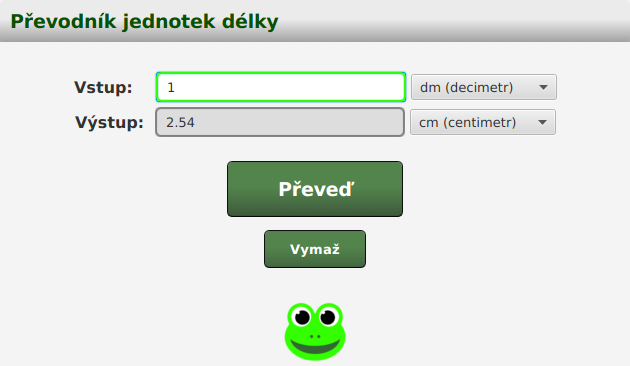
\includegraphics[width=13.5cm]{img/Chyby/Dm.png}
			\end{figure}
			\FloatBarrier
		
		\subsection{Chybné zaokrouhlení}
		Dále u~jednotek decimetry i~palce v~situaci, kdy jsou použity jak na vstupu, tak na výstupu, je hodnota 3 převedena přibližně na 2.9999996, viz \ref{Zaokrouhleni}.
			\begin{figure}[ht!]
				\centering
				\caption{Chybné zaokrouhlení při převodu mezi decimetry}
				\label{Zaokrouhleni}
				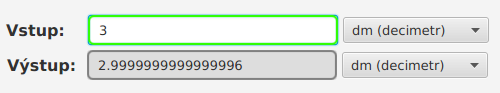
\includegraphics[width=13.5cm]{img/Chyby/Zaokrouhleni.png}
			\end{figure}
			\FloatBarrier
		
		\subsection{Převod záporné hodnoty}
		Při zadání záporné hodnoty pro převod se zobrazí chybová hláška o~záporném čísle, avšak převod se i~tak provede, viz \ref{ZapornaHodnota}.
			\begin{figure}[ht!]
				\centering
				\caption{Převod záporné hodnoty}
				\label{ZapornaHodnota}
				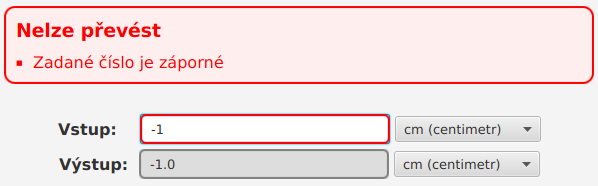
\includegraphics[width=13.5cm]{img/Chyby/ZapornaHodnota.png}
			\end{figure}
			\FloatBarrier
		
		\subsection{Tlačítko Vymaž}
		Tlačítko \emph{Vymaž} nenastaví všem komponentám výchozí hodnoty. Pouze vymaže obsah vstupního pole. Výstupní pole a~výběrové seznamy nadále obsahují hodnoty z~posledního převodu, viz \ref{Vymazani}.
			\begin{figure}[ht!]
				\centering
				\caption{Použití tlačítka Vymaž}
				\label{Vymazani}
				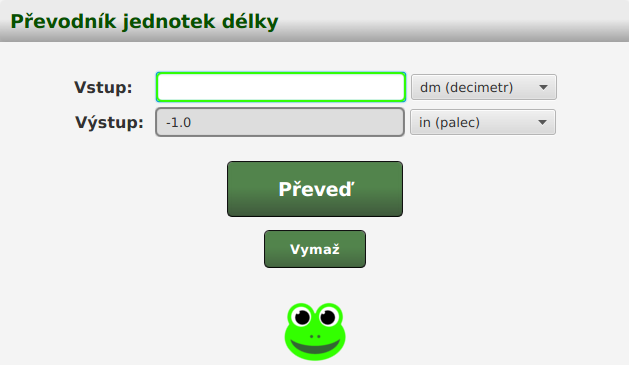
\includegraphics[width=13.5cm]{img/Chyby/Vymazani.png}
			\end{figure}

\chapter{Problémy práce se SikuliX}
Během tvorby testů je možné narazit na různé problémy. Ty, které byly zjištěny během vytváření této práce, jsou zde uvedeny, popsány a~je k~nim nastíněno možné řešení.

	\section{Rozlišení obrazovky}
	Jelikož se SikuliX v~aplikaci orientuje podle screenshotů, je v~danou chvíli závislé na rozlišení, ve kterém byl snímek pořízen. To je z~důvodu, že ještě není implementována funkce, která by měla tento problém odstranit. Pokud se změní rozlišení, nebude daný prvek nalezen, ačkoli bude možné pouhým okem zjistit, že ve skutečnosti přítomen je. Stejný problém nastává i~pokud se změní např. písmo nebo velikost webové stránky s~aplikací a~podobnými změnami vzhledu.
	
	Jedním z~možných řešení je, že si uděláte screenshoty pro různá rozlišení, písma nebo velikosti stránek, případně budete testovat pouze s~jedním daným rozlišením, písmem nebo velikostí stránky.
	
	Nejvhodnější je nastavit v~prohlížeči 100\% velikost stránky. Toho se v~Google Chrome nechá docílit např. tak, že klikneme na ikonku \emph{Menu} a~položku \emph{Lupa} (příp. \emph{Zoom}) nastavíme na 100\%, jak je ukázáno na obrázku \ref{zoom}.
	
	\begin{figure}[ht!]
		\centering
		\caption{Nastavení 100\% velikosti stránky}
		\label{zoom}
		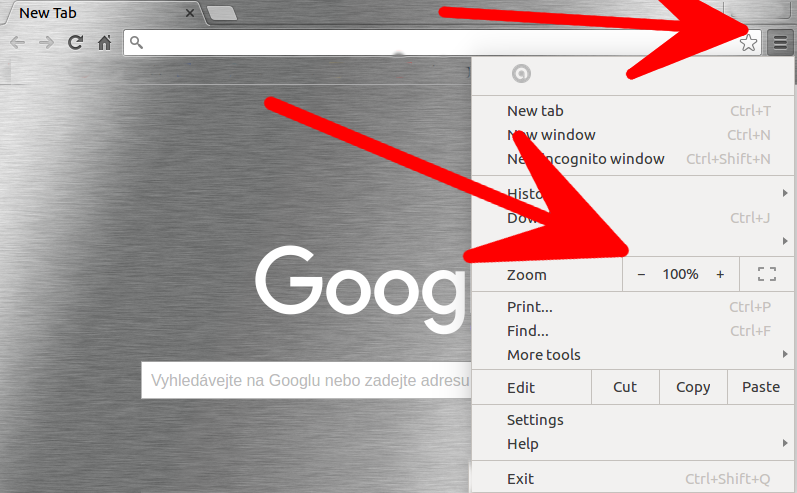
\includegraphics[width=12.5cm]{img/Chyby/zoom.png}
	\end{figure}
	
	\section{Rozměry screenshotů}
	Pokud se v~testu hledá prvek v~závislosti na pozici jiného, je možné, že nebude nalezen. Důvodem mohou být rozdílné rozměry screenshotů v~kombinaci s~použitými metodami hledání -- první prvek nalezneme, ale screenshot druhého je větší, než prohledávaná oblast vymezená rozměry prvního, tudíž nemůže být nalezen. Obrázek \ref{rozmery} demonstruje problém. Pokud budeme hledat červeně vyznačený obrázek, který je vyšší než snímek, ve kterém hledáme, nebude nalezen.
	
	Na snímku je situace, kdy se někde v~záložce \emph{Reklama} nalézá ikona \emph{KIV}. První snímek obrazovky ukazuje výřez záložky \emph{Reklama}. Tento snímek je vysoký x, y pixelů. Druhý, červeně orámovaný snímek již ukazuje hledané logo \emph{KIV} (ve stejném měřítku), ale výška tohoto snímku je (chybně / zbytečně) o~10 pixelů na každou stranu větší, než první snímek.
	
	\begin{figure}[ht!]
		\centering
		\caption{Nesprávné rozměry screenshotů}
		\label{rozmery}
		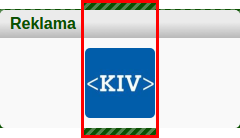
\includegraphics[width=12.5cm]{img/Chyby/reklama.png}
	\end{figure}
	
	\section{Ukazatel myši}
	Při pořizování screenshotů je vhodné vyvarovat se umístění ukazatele myši ve snímané oblasti. Ten se totiž v~průběhu testu v~této oblasti vyskytovat nemusí a~hledaný prvek by tak nemusel být rozpoznán.
	
	Stejně tak je důležité uvědomit si, že na některých platformách se simulováním pohybu myši a~klikáním mění pozice ukazatele. To může vyústit v~problém, pokud je ukazatel umístěn přes hledaný prvek, který tím pádem pravděpodobně nebude rozpoznán. Oba problémy shrnuje obrázek \ref{mys}.
	
	\begin{figure}[ht!]
		\centering
		\caption{Screenshot s~ukazatelem myši}
		\label{mys}
		
\includegraphics[width=6cm]{img/Chyby/mys.png}
	\end{figure}
	
	\section{Nespolehlivé OCR}
	SikuliX poskytuje možnost rozpoznání textu v~obrázcích. Tato funkcionalita je však v~experimentální fázi a~na jejím vývoji se stále pracuje. Je tedy nespolehlivá a~pro naše účely nevhodná. Text v~obrázku buď vůbec nebyl nalezen (pokud se jednalo např. o~jedinou číslici), nebo byl špatně rozpoznán (záměna O~a~0, získána pouze část textu, apod.).
	
	Možným řešením je tedy nasimulovat korektní výstup, provést screenshot a~ten použít pro obrazové rozpoznání správného výsledku.
	
	\section{Nefunkčnost některých metod, tříd}\label{Problemy}
	Java API SikuliX poskytuje třídy a~metody pro práci s~aplikacemi a~jejich okny. Tyto metody a~třídy mají však občas jiné než očekávané chování. Vzhledem k~téměř nulové dokumentaci je toto celkem velký problém.

		\subsection{Pozice a~velikost okna}		
		Konkrétním příkladem je např. to, pokud bychom chtěli testování omezit pouze na okno aplikace. SikuliX je schopno okno s~aplikací najít podle (části) jejího titulku a~přenést jej do popředí. Už ale není schopno získat rozměry a~pozici tohoto okna, ačkoli metody pro tyto funkce existují.
	
		Postup, kterým se dá tato funkcionalita nahradit, je následující. Aplikaci najdeme podle jejího titulku a~necháme ji přenést do popředí. Poté je SikuliX schopné získat pozici a~rozměry okna, které je v~popředí (má tzv. focus), jak je ukázáno v~následujícím kódu.\\[0.2cm]
		\texttt{Region window = App.focusedWindow();\\
		Location minCoord = window.getTopLeft();\\
		Location maxCoord = window.getBottomRight();}
		
		\subsection{Stav aplikace}
		Dále nedokázalo indikovat, že aplikace skončila svůj běh. Pokud jsme tedy použili cyklus \uv{testuj, dokud aplikace běží}, testování pokračovalo i~v~případě, že byla aplikace již ukončena.
	
		Náhradním řešením tedy bylo vytvořit screenshot některé části aplikace, která se nemění a~je vždy v~aplikaci přítomna. Cyklus poté vypadá takto: \uv{testuj, dokud najdeš tuto část aplikace}. To však není řešení absolutní, protože nebude funkční v~případech, kdy se objeví např. dialogové okno, které tuto části zakryje, nebo pokud taková část vůbec neexistuje.
		
		\subsection{Spuštění aplikace}
		Metody pro spuštění aplikace \texttt{App.open("aplikace")}, \texttt{new App(\\"aplikace").open()} a~\texttt{App.run("příkaz")}, které SikuliX poskytuje, fungovaly bez problémů v~OS Linux, avšak v~OS Windows nastal problém. SikuliX nebylo schopné otevřít aplikaci pomocí ani jednoho z~příkazů\\[0.2cm]
		\texttt{App.open("java -jar cesta/k/aplikaci.jar");\\
		new App("java -jar cesta/k/aplikaci.jar").open();\\
		App.run("java -jar cesta/k/aplikaci.jar");}\\[0.2cm]
		Týká se to pouze spouštění aplikace pomocí daného příkazu. Pokud by byla zadána cesta ke spustitelnému souboru (např.: \texttt{cesta/ke/spustitelnemu/\\souboru.exe}), vše proběhlo bez problémů i~za použití těchto metod.
		
		Problém jsem nebyl schopen za pomoci SikuliX vyřešit. Použil jsem proto metodu poskytovanou programovacím jazykem Java, konkrétně\\[0.2cm]
		\texttt{Runtime.getRuntime().exec("java -jar cesta/k/aplikaci.jar");\\
		App application = new App("Titulek aplikace");\\
		application.focus();}
		
		\subsection{Rychlost vykonávaných testů}
		Bylo provedeno srovnání časové náročnosti testů vytvořených pomocí SikuliX a~Selenia pro zjištění přítomnosti statických prvků v~aplikaci. Výsledky jsou uvedeny v~tabulce \ref{casovaNarocnost}, ze které je patrné, že Selenium je rychlejší. Důvodem je nejspíše fakt, že SikuliX obrazově vyhledávalo prvky, kdežto Selenium pouze přistupovalo k~HTML kódu aplikace.
		
		\begin{table}
			\centering
			\caption{Srovnání časové náročnosti testů v~ms}
			\label{casovaNarocnost}
			\begin{tabular}{|l||c|c|c|}
			\hline
			&SikuliX&\shortstack{\\Selenium --\\headless browser}&\shortstack{Selenium --\\Firefox}\\\hline\hline
			Label \emph{Vstup:}&125&122&114\\\hline
			Vstupní textové pole&415&0&105\\\hline
			Vstupní výběrový seznam&165&0&117\\\hline
			Label \emph{Výstup:}&128&66&113\\\hline
			Výstupní textové pole&152&0&117\\\hline
			Výstupní výběrový seznam&449&0&101\\\hline
			Tlačítko \emph{Převeď}&144&1&145\\\hline
			Tlačítko \emph{Vymaž}&332&0&130\\\hline
			\end{tabular}
		\end{table}

\chapter{Monkey testy}
Princip monkey testování byl již zmíněn v~kapitole \ref{MonkeyTestovani}. Zde bude problematika popsána podrobněji a~bude ukázán jeden konkrétní monkey test vytvořený pomocí SikuliX.

Dle \citep{Patton} existují tři druhy monkey testů (\uv{cvičených opic}) lišících se svou inteligencí -- co umí, jaké mají povědomí o~aplikace apod. Jejich vlastnosti a~rozdíly jsou popsány v~následujících částech.

	\section{Hloupá opice}
	Nejjednodušším případem cvičené opice je hloupá opice. Ta neví vůbec nic o~testované aplikace, jen náhodně kliká a~píše na klávesnici. Software, který na počítači běží, není schopný rozlišit cvičenou opici od skutečného člověka, snad jen, že opice by měla akce vykonávat rychleji.
	
	Na první pohled se zdá, že takovýto přístup nemůže najít žádné chyby. Opak je ale pravdou, neboť jak se ukazuje, pokud máme dostatek času a~pokusů, opice až překvapivě často vytvoří jakousi posloupnost akcí, která povede k~havárii aplikace. Na tuto posloupnost nejspíše programátoři ani testeři vůbec nepomysleli, proto nebyla tato chyba nalezena dříve.
	
	Další možnou chybou, kterou může i~hloupá opice zjistit, jsou úniky paměti. Pokud totiž necháme opici pracovat přes noc, poběží software několik hodin (případně můžeme nechat běžet i~několik dní) a~případné problémy se tak mohou projevit.
	
	\section{Zpola inteligentní opice}
	Pokud hloupou opici doplníme o~několik funkcí navíc, zvýšíme její inteligenční kvocient na zpola inteligentní opici. Jednou z~těchto funkcí je zaznamenávání prováděných činností do souboru -- logu. Díky tomu jsme poté schopni přesněji identifikovat, co se dělo těsně před selháním aplikace.
	
	Další takovou funkcí je, aby opice pracovala pouze s~testovanou aplikací. Pokud kliká a~píše kamkoli na obrazovce, jednou by zvolila i~možnost vypnutí počítače, čímž bychom ztratili drahý čas na testování. V~jiném případě by zvolila možnost ukončit aplikaci, ale jelikož by si toho nebyla vědoma, pokračovala by v~klikání a~psaní na vše možné, co se vyskytuje na obrazovce. Zjištění, zda je ještě aplikace spuštěná, se řadí k~těmto funkcím také.
	
	Vhodná je i~ta možnost, která dovolí opici aplikaci po selhání znovu spustit a~pokračovat tak v~testování.
	
	\section{Inteligentní opice}
	Dalším evolučním krokem je inteligentní opice. Ta do klávesnice \uv{nebuší} zcela náhodně, ale uvědomuje si následující věci:
		\begin{itemize}
			\item kde se nachází,
			\item co na tomto místě může dělat,
			\item kam může přejít,
			\item kde již byla,
			\item jestli je to, co vidí, opravdu správné.
		\end{itemize}
	Opice si je tedy vědoma všech (minimálně některých) stavů aplikace a~přechodů mezi nimi. Díky tomu dokáže s~programem pracovat přibližně stejně, jako případný uživatel, jen mnohem rychleji.
	
	Inteligentní opice se však nemusí omezovat jen na hledání chyb, ale mohou také kontrolovat výsledky činností aplikace, správnost výstupů apod. Pokud je navíc schopna vykonávat konkrétní testovací případy, může nalézat poměrně velké množství chyb.
	
	\section{Monkey test pomocí SikuliX}
	Pro účely této práce byl vytvořen jeden monkey test prováděný nad aplikací \emph{Kalkulačka}. Cvičená opice, která jej provádí, je zpola inteligentní -- omezuje se na práci s~oknem aplikace, zapisuje akce do logu a~je si vědoma toho, zda je ještě aplikace spuštěná.
	
	Z~důvodů uvedených v~kapitole \ref{Problemy}, hlavně zhoršenou schopností zjišťovat pozici a~velikost okna aplikace a~její stav, se SikuliX jeví jako nevhodný pro tvorbu tohoto typu testů.
	
	Konkrétní příklad v~kódu \ref{Monkey} běží tak dlouho, dokud existuje statická část aplikace. Ve smyčce poté získá pozici a~velikost jejího okna. Vygeneruje náhodná čísla pro souřadnice vykonávané akce a~další číslo pro určení konkrétní akce (kliknutí, dvojkliknutí, kliknutí pravým tlačítkem, vložení textu případně stisknutí kláves). 
	
	\begin{lstjava}{caption={Monkey test vytvořený pomocí SikuliX}, label={Monkey}}
@Test
public void MonkeyTest01() throws FindFailed {
  Random gen = new Random();
  while (s.exists(title) != null) {
    window = App.focusedWindow();
    Location minCoord = window.getTopLeft();
    Location maxCoord = window.getBottomRight();
    int random = gen.nextInt(5);
    int x = gen.nextInt(maxCoord.getX()), y = gen.
      nextInt(maxCoord.getY());
    while (x < minCoord.getX()) x = gen.nextInt(
      maxCoord.getX());
    while (y < minCoord.getY()) y = gen.nextInt(
      maxCoord.getY());
    switch (random) {
      case 0: // Click
        window.click(new Location(x, y));
        break;
      case 1: // Double-click
        window.doubleClick(new Location(x, y));
        break;
      case 2: // Right click
        window.rightClick(new Location(x, y));
        break;
      case 3: // Paste
        if (gen.nextInt(2) == 1) window.click(new
          Location(x, y));
        String s = randomString(gen);
        window.paste(new Location(x, y), s);
        logger.info("PASTE \"" + s + "\" on [" + x +
          ", " + y + "]");
        break;
      case 4: // Type
        if (gen.nextInt(2) == 1) window.click(new
          Location(x, y));
        window.type(new Location(x, y),
          randomString(gen));
        break;
    }
  }
}
\end{lstjava}

\chapter{Automatizace nástrojem}
Podle \citep{SikuliX} je SikuliX primárně nástroj pro automatizaci činností. Je vhodný pro kohokoli, kdo provádí opakovaně některé monotónní činnosti jako denní práce s~aplikacemi nebo webovými stránkami, hraní her, administrace IT systémů a~sítí apod.

Zde ukážeme možnost automatizace takového procesu na konkrétním příkladu, viz kód \ref{automatizace}. Jedná se o~zapnutí a~případné přihlášení (pokud jsme se během sezení již nepřihlašovali) do aplikace \emph{TestLink} instalované podle postupu v~podkladech k~přednáškám KIV/OKS, viz \citep{Herout}.

Postup je ve své podstatě identický jako při vytváření testovacích případů. Jediným rozdílem je, že nebudeme používat knihovnu \emph{JUnit}, ale skript vytvoříme jako samostatný program v~Javě. Každý si ve skriptu musí upravit cestu k~\emph{Bitnami TestLink Stack Manager Tool}, login a~heslo.

\begin{lstjava}{caption={Automatizace spuštění a přihlášení do aplikace \emph{TestLink}}, label={automatizace}}
public static void main(String[] args) {
  Logger logger = LogManager.getLogger();

  Settings.MoveMouseDelay = 0;
  Debug.setLogger(logger);
  Debug.setLoggerAll("info");

  Screen s = new Screen();
  try {
    Runtime.getRuntime().exec("cesta/k/TestLink/manager/
      tool");
    App application = new App("TestLink");
    application.focus();
    s.wait("png/goToApp.png", 5);
    s.click("png/goToApp.png");
    if (s.exists("png/startServers.png") != null) s.
      click("png/startServers.png");
    application = new App("Chrome");
    application.focus();
    s.wait("png/access.png", 50);
    s.click("png/access.png");
    if (s.exists("png/login.png") != null) {
      s.find("png/login.png").below(20).click();
      s.paste("login");
      s.click("png/login.png");
      s.find("png/pass.png").below(20).click();
      s.paste("password");
      s.type(Key.ENTER);
    }
  } catch (IOException | FindFailed e) {
    s.capture().save("errors", screenshotName());
    logger.error(e.getMessage());
  }
}
\end{lstjava}

\chapter{Statistika}
V~této práci bylo vytvořeno 103 testů (každý pro webovou a~JavaFX aplikaci, dohromady tedy 206 testů). Počet snímků potřebných pro vytvoření testů bylo 74 (každý pro webovou a~JavaFX aplikaci jak na Linux, tak na Windows, celkem tedy 296 snímků). Dohromady bylo vytvořeno více než 330 souborů a~napsáno více než 7350 řádek zdrojového kódu.
		
\chapter{Závěr}
V~práci jsou popsány některé metody testování grafického uživatelského rozhraní a~také základní důvody používání těchto metod. V~první části práce je proveden kvalifikovaný průzkum existujících a~dostupných nástrojů, které je možné k~testování GUI využít.

Byly vybrány tři nástroje, jejichž stručná charakteristika je uvedena v~teoretické části práce. Dále bylo navrženo multikriteriální hodnocení a~provedeno podrobné porovnání zvolených nástrojů. Multikriteriální hodnocení má sedm kritérií. Jejich váhy si může zájemce určit sám, viz tabulkový soubor na CD. Podle vah diskutovaných s~vedoucím práce byl vybrán nástroj SikuliX, který byl dále detailně zkoumán.

Možnosti nástroje SikuliX byly okamžitě ověřovány v~připravovaných praktických testech. Aby bylo možné demonstrovat, že SikuliX má širší možnosti pro testování než nástroj pro testování webových aplikaci Selenium, bylo nutné nejdříve připravit identickou desktopovou aplikaci k~již existující webové aplikaci. Podle již existujícího vzoru byly připraveny v~SikuliX dvě kompletní sady testů jak pro desktopovou, tak pro webovou aplikaci. Tento přístup dovoluje porovnat oba dva způsoby testování a~poukázat na případné drobné rozdíly mezi nimi.

Při testování byly využity možnosti frameworku JUnit a~rovněž předpřipravené možnosti SikuliX pro logování, které nebývá v~testování tak běžné. Zde se ale ukazuje, že je výhodné.

Pozornost byla v~práci věnována i~monkey testům a~automatizaci činností, přičemž bylo zjištěno, že obě dvě aktivity se nijak výrazně neodlišují od psaní běžných testů.

V~práci je též stručně porovnána časová náročnost nástrojů, ale je třeba říci, že toto není podstatné kritérium výběru nástroje.

V~této práci bylo vytvořeno dvakrát 103 testů (každý pro webovou a~JavaFX aplikaci, dohromady tedy 206 testů). Počet snímků potřebných pro vytvoření testů byl čtyřikrát 74 (každý pro webovou a~JavaFX aplikaci jak na Linux, tak na Windows, celkem tedy 296 snímků). Dále byl vytvořen jeden monkey test a~jeden skript pro ukázku automatizace činnosti. Dohromady bylo vytvořeno více než 330 souborů a~napsáno více než 7350 řádek zdrojového kódu.

Výsledky práce budou přímo použity pro přípravu jedné z~přednášek předmětu Ověřování kvality softwaru vyučovaného na KIV.
 
% 
% PRO ANGLICKOU SAZBU JE NUTNÉ ZMĚNIT
% CITAČNÍ STYL!
%
\bibliographystyle{csplainnatkiv}
{\raggedright\small
\bibliography{literatura}
}

\chapter*{Příloha A}
\addcontentsline{toc}{chapter}{Příloha A}

	\begin{lstjava}{caption={Další testy Java API}, label={DalsiJavaAPI}}
import org.apache.logging.log4j.LogManager;
import org.apache.logging.log4j.Logger;
import org.junit.AfterClass;
import org.junit.Before;
import org.junit.BeforeClass;
import org.junit.Test;
import org.junit.rules.ErrorCollector;
import org.sikuli.basics.Debug;
import org.sikuli.basics.Settings;
import org.sikuli.script.*;
import javax.swing.*;
import java.time.LocalDateTime;
import static org.junit.Assert.*;

public class Test01 {

  static Logger logger;
  static ErrorCollector collector;
  static Screen s;
  static App prohlizec;
  static boolean run;

  static {
    System.setProperty("log4j.configurationFile",
      "log-konfigurace.xml");
  }

  private String nazevScreenshotu() {
    LocalDateTime l = LocalDateTime.now();
      return l.getYear() + "" + l.getMonthValue() +
        "" + l.getDayOfMonth() + "" + l.getHour() +
        "" + (l.getMinute() < 10 ? "0" + l.
        getMinute() : l.getMinute()) + "" + l.
        getSecond() + "";
  }

  @BeforeClass
  public static void setUpBeforeClass() {
    logger = LogManager.getLogger();

    Settings.OcrTextSearch = true;
    Settings.OcrTextRead = true;
    Debug.setLogger(logger);
    Debug.setLoggerAll("info");

    collector = new ErrorCollector();
    s = new Screen();
    prohlizec = new App("google-chrome");
    prohlizec.open();
    prohlizec.focus();
    run = true;
    }

  @AfterClass
  public static void tearDownAfterClass() {
    JOptionPane.showMessageDialog(null, "Script" +
      " dokoncen");
    prohlizec.close();
  }

  @Before
  public void setUp() {
    try {
      s.wait("png/addressBar.png", 10);
      s.click(new Pattern("png/addressBar.png").
        targetOffset(100, 0));
      s.paste("http://oks.kiv.zcu.cz/Prevodnik");
      s.type(Key.ENTER);
      s.wait("png/zalozkaPrevodnik.png", 5);
    } catch (Exception e) {
      run = false;
      s.capture().save("errors", nazevScreenshotu());
      logger.error(e.getMessage());
    }
  }

  @Test
  public void testPorovnejText() {
    if (run) {
      try {
        s.click("png/zalozkaPrevodnik.png");
        s.wait("png/tlacitkoPreved.png", 5);
        s.paste("png/vstup.png", "1");
        Match m = s.find("png/jednotky.png");
        m.setTargetOffset(-27, -18);
        m.click();
        s.findText("(metr)").click();
        s.click(new Pattern("png/jednotky.png").
          targetOffset(-27, 18));
        s.find("png/dm.png").click();
        s.click("png/tlacitkoPreved.png");
        String t = s.find("png/vystup.png").right(
          100).text();
        assertEquals(10, Double.parseDouble(t),
          0.01);
      } catch (FindFailed | AssertionError e) {
        s.capture().save("errors",
          nazevScreenshotu());
        logger.error(e.getMessage());
        fail(e.getMessage());
      }
    } else {
      run = true;
      logger.error("setUp neuspesny");
      fail("setUp neuspesny");
    }
  }

  @Test
  public void testPorovnejObraz() {
    if (run) {
      try {
        s.click("png/zalozkaPrevodnik.png");
        s.wait("png/tlacitkoPreved.png", 5);
        s.paste("png/vstup.png", "1");
        s.click(new Pattern("png/jednotky.png").
          targetOffset(-27, -18));
        s.click("png/inch.png");
        s.click("png/tlacitkoPreved.png");
        assertTrue(s.exists("png/vysledek.png") !=
          null);
      } catch (FindFailed | AssertionError e) {
        s.capture().save("errors",
          nazevScreenshotu());
        logger.error(e.getMessage());
        fail(e.getMessage());
      }
    } else {
      run = true;
      logger.error("setUp neuspesny");
      fail("setUp neuspesny");
    }
  }

  @Test
  public void testZkontrolujOdkazObrazekKiv() {
    if (run) {
      try {
        s.click("png/logoKiv.png");
        assertTrue(s.exists("png/zahlaviKiv.png") !=
          null);
      } catch (FindFailed | AssertionError e) {
        s.capture().save("errors",
          nazevScreenshotu());
        logger.error(e.getMessage());
        fail(e.getMessage());
      }
    } else {
      run = true;
      logger.error("setUp neuspesny");
      fail("setUp neuspesny");
    }
  }

  @Test
  public void testChyba() {
    if (run) {
      try {
        s.wait("png/tlacitkoPreved.png", 5);
        s.paste("png/vstup.png", "1");
        s.click(new Pattern("png/jednotky.png").
          targetOffset(-27, -18));
        s.findText("(metr)").click();
        s.click("png/tlacitkoPreved.png");
        String t = s.find("png/vystup.png").right(
          100).text();
        assertEquals(100, Double.parseDouble(t),
          0.01);
      } catch (FindFailed | AssertionError e) {
        s.capture().save("errors",
          nazevScreenshotu());
        logger.error(e.getMessage());
        fail(e.getMessage());
      }
    } else {
      run = true;
      logger.error("setUp neuspesny");
      fail("setUp neuspesny");
    }
  }
}
	\end{lstjava}
\end{document}
